
\chapter{Experiments} % Main chapter title

\section{Training Details}

The models are trained on the dataset \textit{synthetic-50-5} with 3000 scenes mentioned in chapter \ref{ch:04}. Each scene has a depth map with dimension $ 128\times 128 $ in height and width, an image with dimension $ 128\times 128 $. The depth map is converted from the 3D vertex map as introduced in chapter \ref{ch:04}. The light map is computed from the vertex map and the known light position. We create a tensor in PyTorch containing the vertex map, image, and light direction for each scene and consider it as a training case. Thus, 3000 scenes correspond to 3000 training cases. For each scene, there is a corresponding ground truth normal map for loss calculation and evaluation. Figure \ref{fig:test-scene} shows some of the training cases. Note that the position of the objects is not always placed naturally on the stage, but with a random rotation in the X, Y and Z axes.

% test scene
\begin{figure}[H]
	\centering
	\captionsetup{width=\linewidth}
	\begin{subfigure}[b]{0.24\linewidth}
		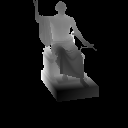
\includegraphics[width=\linewidth]{./Figures/test_scenes/03094.depth0.png}
	\end{subfigure}
	\begin{subfigure}[b]{0.24\linewidth}
		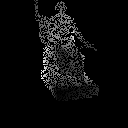
\includegraphics[width=\linewidth]{./Figures/test_scenes/03094.depth0_noise.png}
	\end{subfigure}
	\begin{subfigure}[b]{0.24\linewidth}
		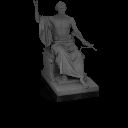
\includegraphics[width=\linewidth]{./Figures/test_scenes/03094.image0.png}
	\end{subfigure}
	\begin{subfigure}[b]{0.24\linewidth}
		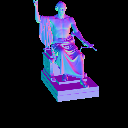
\includegraphics[width=\linewidth]{./Figures/test_scenes/03094.normal0.png}
	\end{subfigure}
	
	
	\begin{subfigure}[b]{0.24\linewidth}
		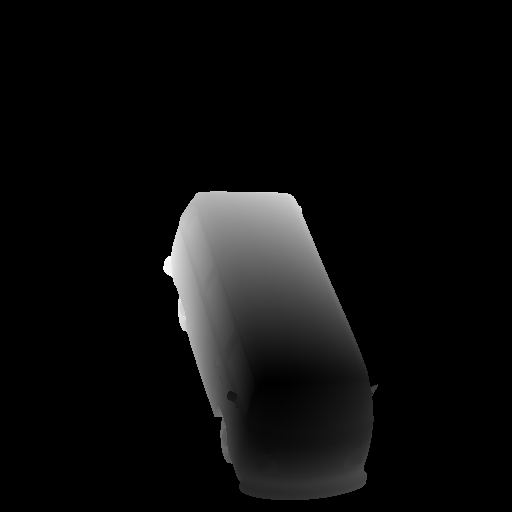
\includegraphics[width=\linewidth]{./Figures/test_scenes/05126.depth0.png}
		\caption{Depth Map}
	\end{subfigure}
	\begin{subfigure}[b]{0.24\linewidth}
		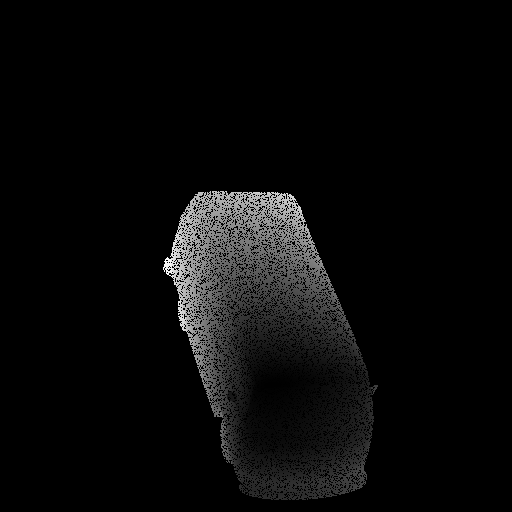
\includegraphics[width=\linewidth]{./Figures/test_scenes/05126.depth0_noise.png}
		\caption{Added noise}
	\end{subfigure}
	\begin{subfigure}[b]{0.24\linewidth}
		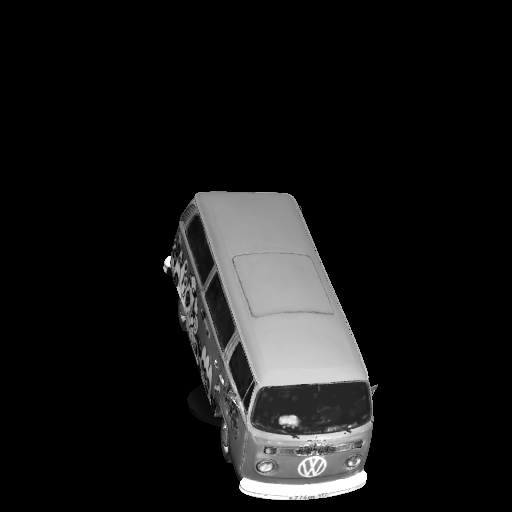
\includegraphics[width=\linewidth]{./Figures/test_scenes/05126.image0.png}
		\caption{Image}
	\end{subfigure}
	\begin{subfigure}[b]{0.24\linewidth}
		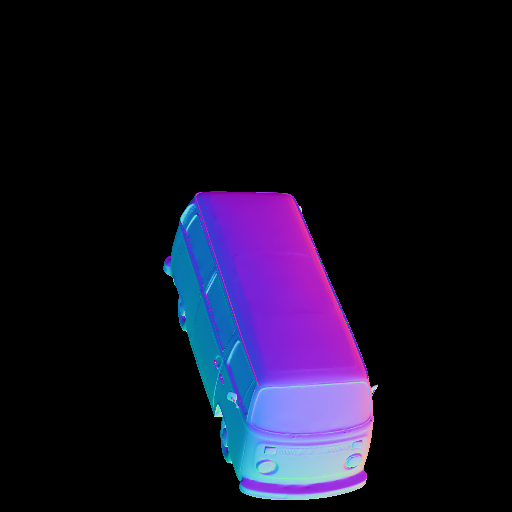
\includegraphics[width=\linewidth]{./Figures/test_scenes/05126.normal0.png}
		\caption{Normal Map}
	\end{subfigure}
	\decoRule
	\caption{Some of the evaluation scenes during the training. The objects from top to bottom rows: \textit{ Washington}, \textit{Bus}}
	\label{fig:test-scene}
\end{figure}


Besides the 3000 training scenes, 100 additional scenes with 5 different object models are used as evaluation dataset during the training. They are evaluated in each epoch. 

For the training parameters, we set the training pipeline with a batch size of 8, since we found that a higher batch size decreases the final performance.  Adam Optimizer (\cite{adam}), learning rate starting at $ 1\times10^{-3} $, it will decrease at epoch 8 with learning decay factor 0.5. The model is trained using PyTorch 1.10.0a0, CUDA 11.4.1, GPU with an NVIDIA GEFORCE RTXA 6000. It takes 14 hours to train the GCNN and 35 hours to train the Trip-Net. We stop training when the angular error of the normal map stops decreasing.

\begin{flushright}
	
\end{flushright}
The \textit{GCNN} is the base model of the whole work. The architecture is described in \ref{sec:gcnn}. We use a single \textit{GCNN} to estimate surface normals as a geometry-based approach. It uses a vertex map as input. To verify the applicability of the skip-connection and gated-convolution layers, we trained two additional models for comparison. 
In the first model, we replace all gated layers with default convolutional layers in the network, but keep all other settings and give it the name \textit{CNN}. It is used to compare the performance between the gated layer and the default convolutional layer for our normal inference task. As mentioned in \ref{ch:03}, the gated layer is designed to process noisy input. Since the entire vertex map in the dataset was noisy, the \textit{GCNN} should outperform \textit{CNN}. 
Another model called \textit{NOC} is used to check skip connections, which simply removes the skip connections in the network but leaves the other settings unchanged. Its purpose is to show to what extent the performance of the model is improved by skipping connections. We use Reversed Huber Loss as a loss function during training. We have found that it gives a better final error compared to L2 loss. 



\begin{table}[H]
	\centering
	\captionsetup{width=\linewidth}
	\begin{tabular}{l | l l l l l }
		\toprule
		\tabhead{Model} & $ \# $\textbf{Total} &\textbf{ V-P} & \textbf{L-P} & \textbf{I-P} & \tabhead{Size /MB}\\
		\midrule
		\hline
		CNN 					& 17 & 32 & - & - & 25.5 \\
		\hline
		NOC 					& 32 & 32 & - & - & 30.6 \\
		\hline
		GCNN 					& 32 & 32 & - & - & 45.8 \\
		\bottomrule
	\end{tabular}
	\caption{GCNN model information. The V-P, L-P, and I-P columns indicate the number of convolutional layers in the vertex pipe, light pipe, and image pipe, respectively. Note that a gated convolution layer consists of 2 standard layers and is therefore counted as 2.}	
	\label{tab:gcnn-eval-mean}
\end{table}


The trip-net model uses a triple GCNN architecture with 4 fusions, which is more difficult to train. It takes the calibrated illuminated RGB-D images as input to estimate the surface normal map. When we train this model, we take the GCNN model as the baseline to observe the advantages of the illuminated information with the trip-net architecture.
We also examined the optimal fusion times of the Trip-Net to determine a possible simplification of the model. A set of similar models was trained with the same settings but different fusion times, denoted Trip-Net-F$ x $, where $ x $ denotes the fusion times. We score the fusion times from 1 to 4. For the learning rate, we initially set $ 1e-3 $. This fits the GCNN model well, but leads to a loss explosion in the trip-net. Therefore, we set a learning rate schedule with an additional decay step at epoch 8. The decay factor is $ 0.5$. The batch size is set to 8.

During training, we found that the trip-net with 4 fusions converges significantly faster than models with fewer fusion times. However, model F3 with three times fusion converges slower than F4, but ends up with a similar loss of score as F4 (see Qualitative Evaluation). Models F1 and F2 are relatively less accurate than the other two models, but the sacrifice of accuracy results in a relatively lighter model. Since they have fewer fusion times, the corresponding upsampling layers in the image and light pipes can also be removed. The model can be trained faster, and the size is also smaller. Table \ref{tab:trip-net-size-compare} contains a comparison of the size of different models.



\begin{table}[H]
	\centering
	\captionsetup{width=\linewidth}
	\begin{tabular}{l | l l l l l }
		\toprule
		\tabhead{Model} & $ \# $\textbf{Total} &\textbf{ V-P} & \textbf{L-P} & \textbf{I-P} & \tabhead{Size /MB}\\
		\midrule
		Trip-Net-F1F  			& 88 &  40 & 24 & 24 & 106\\ 
		\hline
		Trip-Net-F2F 			& 92 & 40 & 26 & 26 & 137 \\ 
		\hline
		Trip-Net-F3F 			& 96 & 40 & 28 & 28 & 167 \\
		\hline
		Trip-Net 				& 100 & 40 & 30 & 30 & 198\\
		\bottomrule
	\end{tabular}
	\caption{Trip-Net Model information. Columns V-P, L-P and I-P represent the number of convolution layers in vertex pipe, light pipe and image pipe respectively. Note that one gated convolution layer is constructed with 2 standard layers, thus it is counted as 2. }	
	\label{tab:trip-net-size-compare}
\end{table}


\section{Quantitative Evaluation on 6 Metrics}
We evaluated our models on a synthetic dataset with a resolution of $ 128 by $ 128. 
Based on the metrics proposed by \cite{geometry_based_solution}, 6 different metrics are used for the evaluation. Note that the vertex map input is only semi-dense. One of the advantages of the GCNN architecture is that it is robust to noisy input, so all points, including missing points in the input vertex map, are considered in the evaluation. We use $\tilde{\textbf{N}}$ for the estimated normal map, $ \textbf{N} $ for the ground-truth normal map, $ P $ for the \textit{set} of valid points, \textit{ValidNum} for the number of valid points. \textit{abs} is a function to calculate the absolute value of the given values, \textit{median} is a function to calculate the median value of a given \textit{set}.



\paragraph{Average Angle Error Metric (AAE)}
The metric calculates the average absolute angular error for each point between the inferred normal and the ground-truth normal map.
%% https://www.cuemath.com/geometry/angle-between-vectors/
\[ 
AAE = \frac
{1}
{ValidNum} \cdot \sum_{i\in P}  \left|   \arccos \frac{\textbf{N}_{i}\cdot \tilde{\textbf{N}}_{i}} {| \textbf{N}_{i} |  |\tilde{\textbf{N}}_{i}|  } \cdot  \frac{180}{\pi}   \right| 
\]

\paragraph{Median Angle Error Metric (MED)}
The metric calculates the median of the absolute angular error of all points in the normal map.

\[ 
MED = 
\text{Median}   \left( \Bigg\{ \left|\arccos \frac{\textbf{N}_{i}\cdot \tilde{\textbf{N}}_{i}} {| \textbf{N}_{i} |  |\tilde{\textbf{N}}_{i}|  } \right| \text{for}\ i \in P   \Bigg\}\right)
\]

\paragraph{5 Degree Error Metric ($ E_5 $)}
The metric calculates the percentage of predicted normals that have an error less than $ 5^\circ $ compared to ground truth. First, the number of normals that have an error less than $ 5^\circ $ ($ D_5 $) is calculated.
\[
D_5 = \sum_{i\in P} \left( \text{abs}\left(   \arccos \frac{\textbf{N}_{i}\cdot \tilde{\textbf{N}}_{i}} {| \textbf{N}_{i} |  |\tilde{\textbf{N}}_{i}|  } \cdot  \frac{180}{\pi}   \right) < 5 \right)
\]
Then the percentage of normals that have error less than $ 5^\circ $ ($ E_5 $) is calculated.
\[ 
E_5 = \frac{D_5}{ValidNum}\times 100\%
\]


\paragraph{11.5 Degree Error Metric ($ E_{11.5} $)}
The metric calculates the percentage of predicted normals that have an error less than $ 11.5^\circ $ compared to ground truth. First, the number of normals that have an error less than $ 11.5^\circ $ ($ D_{11.5} $) is calculated.

\[
D_{11.5} = \sum_{i\in P} \left( \text{abs}\left(   \arccos \frac{\textbf{N}_{i}\cdot \tilde{\textbf{N}}_{i}} {| \textbf{N}_{i} |  |\tilde{\textbf{N}}_{i}|  } \cdot  \frac{180}{\pi}   \right) < 11.5 \right)
\]
Then the percentage of normals that have error less than $ 11.5^\circ $ ($ E_{11.5} $) is calculated.
\[ 
E_{11.5} = \frac{D_{11.5}}{ValidNum}\times 100\%
\]

\paragraph{22.5 Degree Error Metric ($ E_{22.5} $)}
The metric calculates the percentage of predicted normals that have an error less than $ 22.5^\circ $ compared to ground truth. First, the number of normals that have an error less than $ 22.5^\circ $ ($ D_{22.5} $) is calculated.

\[
D_{22.5} = \sum_{i\in P} \left( \text{abs}\left(   \arccos \frac{\textbf{N}_{i}\cdot \tilde{\textbf{N}}_{i}} {| \textbf{N}_{i} |  |\tilde{\textbf{N}}_{i}|  } \cdot  \frac{180}{\pi}   \right) < 22.5 \right)
\]
Then the percentage of normals that have error less than $ 22.5^\circ $ ($ E_{22.5} $) is calculated.
\[ 
E_{22.5} = \frac{D_{22.5}}{ValidNum}\times 100\%
\]


\paragraph{30 Degree Error Metric ($ E_{30} $)} 
The metric calculates the percentage of predicted normals that have an error less than $ 30^\circ $ compared to ground truth. First, the number of normals that have an error less than $ 30^\circ $ ($ D_{30} $) is calculated.

\[
D_{30} = \sum_{i\in P} \left( \text{abs}\left(   \arccos \frac{\textbf{N}_{i}\cdot \tilde{\textbf{N}}_{i}} {| \textbf{N}_{i} |  |\tilde{\textbf{N}}_{i}|  } \cdot  \frac{180}{\pi}   \right) < 30 \right)
\]
Then the percentage of normals that have error less than $ 30^\circ $ ($ E_{30} $) is calculated.
\[ 
E_{30} = \frac{D_{30}}{ValidNum}\times 100\%
\]

We evaluated our trained models on \textit{synthetic-50-5}. In the test dataset, 5 objects are considered. They are: \textit{Baoshanlu}, \textit{Bus}, \textit{Dragon}, \textit{Garfield} and \textit{Washington}. Each object has 20 scenes with a total of 100 scenes for 5 objects. The test objects are not present in the training dataset. We evaluate all the presented models on the test dataset, to fit them into a table, the names of each model are simplified. The model \textit{SVD} uses the SVD optimization method, the model \textit{NOC} is the no-skip connection version of \textit{GCNN}, \textit{CNN} is the CNN version of \textit{GCNN}. \textit{F1}, \textit{F2}, \textit{F3}, \textit{F4} are the fusion times in the \textit{Trip-Net}. 




When evaluating the \textit{GCNN} models, we take \textit{SVD} model with an optimal neighborhood size as baseline. \textit{NOC} and \textit{CNN} are used to verify the performance of \textit{GCNN} model. When evaluate the \textit{F1}-\textit{F4} models, we can take \textit{GCNN} model as baseline. 

From the table we can see that all the learning based approaches achieves a better result than SVD approach. In the 30 degrees error metric, GCNN based approach achieves 95 \% accuracy whereas Trip-Net is even higher, some of the models like \textit{dragon} achieves 98\%. The best performance is around 90\%, 75 \%, 45 \% in $ 22.5^\circ $, $ 11.5^\circ $ and $ 5^\circ $ degrees error metrics respectively. Another notable result is the close performance of F3 and F4 models, where they achieves a very comparable performance. We also found that during the training, F4 model converges faster than F3, but F3 in the end achieves a similar loss with model F4. However, based on the $ 30^\circ $, $ 22.5^\circ $, $ 11.5^\circ $ metrics, we can still see that F4 model gives a more stable performance with less high error normals. This is reasonable since the last fusion in the original resolution provides more high resolution information to the models.



In evaluating the \textit{GCNN} models, we take the \textit{SVD} model with an optimal neighborhood size as the baseline. \textit{NOC} and \textit{CNN} are used to check the performance of the \textit{GCNN} model. When evaluating the \textit{F1}-\textit{F4} models, we can take the \textit{GCNN} model as a baseline. 

From the table, it can be seen that all learning-based approaches achieve a better result than the \textit{SVD} approach. In the 30-degree error metric, the GCNN-based approach achieves 95\% accuracy, while Trip-Net is even higher and some models such as \textit{dragon} achieve 98\%. 
The best performance is 90\%, 75\%, 45\% in the $ 22.5^\circ $, $ 11.5^\circ $ and $ 5^\circ $ degree error metric, respectively. Another notable result is the close relationship between the F3 and F4 models, which achieve very comparable performance. We also found that model F4 converges faster than F3 during training, but F3 ends up achieving a similar loss as model F4. However, using the metrics $ 30^\circ $, $ 22.5^\circ $ and $ 11.5^\circ $, we can see that the F4 model has a more stable performance with less high error normals. This is reasonable since the last fusion at the original resolution provides more high-resolution information to the models.


%% mean metric
\begin{table}[H]
	\centering
	\captionsetup{width=\linewidth}
	\begin{tabular}{l | l | l l l | l l l l }
		\toprule
		\tabhead{Object} & \tabhead{SVD} & \tabhead{GCNN} & \tabhead{NOC} & \tabhead{CNN} & \tabhead{F1}& \tabhead{F2}& \tabhead{F3}& \tabhead{F4}\\
		\midrule
		Baoshanlu  		& 35.66 & 11.09 & 13.58 & 15.55 & 11.22 & 10.36 &\textbf{ 9.77 }& 9.80 \\ 
		\hline
		Bus 			& 31.93 & 7.79 & 8.95 & 11.93 & 7.49 & 7.85 & \textbf{7.30} & 7.62\\ 
		\hline
		Dragon 			& 39.57 & 10.60 & 15.29 & 16.03 & 10.47 & 10.23 & 8.16 &\textbf{ 7.79} \\
		\hline
		Garfield 		& 39.69 & 10.20 & 12.50 & 14.46 & 9.94 & 10.36 & 9.71 &\textbf{ 9.39} \\
		\hline
		Washington 		& 42.83 & 13.43 & 17.59 & 18.71 & 13.32 & 13.40 & 12.62 &\textbf{ 12.60}\\
		\bottomrule
	\end{tabular}
	\caption{Average angular error of the evaluation dataset. \textit{SVD} Neighborhood size $ k=2 $}	
	\label{tab:eval-mean}
\end{table}

%% median metric
\begin{table}[H]
	\centering
	\captionsetup{width=\linewidth}
	\begin{tabular}{l | l | l l l | l l l l }
		\toprule
		\tabhead{Object} & \tabhead{SVD} & \tabhead{GCNN} & \tabhead{NOC} & \tabhead{CNN} & \tabhead{F1}& \tabhead{F2}& \tabhead{F3}& \tabhead{F4}\\
		\midrule
		Baoshanlu  		& 34.06 & 8.86 & 10.82 & 13.25 & 8.95 & 8.02 & 7.54 &\textbf{ 7.50} \\ 
		\hline
		Bus 			& 34.14 & 4.44 & 5.02 & 8.69 & 4.11 & 4.58 & \textbf{3.65 }& 4.47 \\ 
		\hline
		Dragon 			& 36.43 & 7.62 & 11.10 & 13.26 & 7.60 & 7.12 & 5.87 &\textbf{ 5.52} \\
		\hline
		Garfield 		& 37.60 & 6.40 & 8.90 &11.31 & 6.30 & 6.72 & 6.21 & \textbf{6.04 }\\
		\hline
		Washington 		& 36.89 & 7.64 & 11.38 & 13.64& 7.49 & 7.60 &\textbf{ 7.03 }& 7.25\\
		\bottomrule
	\end{tabular}
	\caption{Median angular error of the evaluation dataset. \textit{SVD} Neighborhood size $ k=2 $}	
	\label{tab:eval-median}
\end{table}


%% 5 degree metric
\begin{table}[H]
	\centering
	\captionsetup{width=\linewidth}
	\begin{tabular}{l | l | l l l |l l l l }
		\toprule
		\tabhead{Object} & \tabhead{SVD} & \tabhead{GCNN} & \tabhead{NOC} & \tabhead{CNN} & \tabhead{F1}& \tabhead{F2}& \tabhead{F3}& \tabhead{F4}\\
		\midrule
		Baoshanlu  		& 0.01 & 0.25 & 0.18 & 0.11 & 0.24 & 0.31 &\textbf{ 0.33 }& 0.32\\ 
		\hline
		Bus 			& 0.00 & 0.56 & 0.50 & 0.23 & 0.59 & 0.54 & \textbf{0.63 }& 0.55 \\ 
		\hline
		Dragon 			& 0.00 & 0.31 & 0.17 & 0.10 & 0.31 & 0.34 & 0.43 &\textbf{ 0.46}\\
		\hline
		Garfield 		& 0.00 & 0.41 & 0.27 & 0.14 & 0.42 & 0.39 & 0.42 & \textbf{0.43}\\
		\hline
		Washington 		& 0.00 & 0.38 & 0.26 & 0.10 & 0.36 & 0.36 & \textbf{0.40 }& 0.37\\
		\bottomrule
	\end{tabular}
	\caption{Percentage of error of less than 5 degrees of the evaluation data set. \textit{SVD} Neighborhood size $ k=2 $}	
	\label{tab:eval-5d}
\end{table}


%% 11.5 degree metric
\begin{table}[H]
	\centering
	\captionsetup{width=\linewidth}
	\begin{tabular}{l | l | l l l | l l l l }
		\toprule
		\tabhead{Object}  & \tabhead{SVD} & \tabhead{GCNN} & \tabhead{NOC} & \tabhead{CNN} & \tabhead{F1}& \tabhead{F2}& \tabhead{F3}& \tabhead{F4}\\
		\midrule
		Baoshanlu  		& 0.03 & 0.62 & 0.52 & 0.41 &  0.62 & 0.66 &\textbf{ 0.69 }& \textbf{0.69}\\ 
		\hline
		Bus 			& 0.05 & 0.81 & 0.78 & 0.65 & 0.83 & 0.82 & \textbf{0.83 }&\textbf{ 0.83 }\\ 
		\hline
		Dragon 			& 0.02 & 0.69 & 0.51 & 0.40 & 0.70 & 0.71 & 0.79 & \textbf{0.81}\\
		\hline
		Garfield 		& 0.03 & 0.72 & 0.62 & 0.51 &0.73 & 0.71  & 0.74 &\textbf{ 0.75}\\
		\hline
		Washington 		& 0.02 & 0.62 & 0.50 & 0.40 & 0.63 & 0.62 & 0.64 & \textbf{0.65}\\
		\bottomrule
	\end{tabular}
	\caption{Percentage of error of less than 11.5 degrees of the evaluation data set. \textit{SVD} Neighborhood size $ k=2 $}	
	\label{tab:eval-11d}
\end{table}



%% 22.5 degree metric
\begin{table}[H]
	\centering
	\captionsetup{width=\linewidth}
	\begin{tabular}{l | l | l l l | l l l l }
		\toprule
		\tabhead{Object}  & \tabhead{SVD} & \tabhead{GCNN} & \tabhead{NOC} & \tabhead{CNN} & \tabhead{F1}& \tabhead{F2}& \tabhead{F3}& \tabhead{F4}\\
		\midrule
		Baoshanlu  		& 0.18 & 0.90 & 0.84 & 0.79 & 0.90 & 0.91 &\textbf{ 0.92} &\textbf{ 0.92}\\ 
		\hline
		Bus 			& 0.26 & 0.93 & 0.91 & 0.89 & 0.93 & 0.93 & 0.93 & \textbf{0.94}\\ 
		\hline
		Dragon 			& 0.14 & 0.90 & 0.79 & 0.80 & 0.90 & 0.90 & 0.94 & \textbf{0.95}\\
		\hline
		Garfield 		& 0.13 & 0.89 & 0.86 & 0.84 & 0.90 & 0.89 &\textbf{ 0.91} &\textbf{ 0.91}\\
		\hline
		Washington 		& 0.14 & 0.81 & 0.72 & 0.72 & 0.81 & 0.81 & \textbf{0.83} &\textbf{ 0.83}\\
		\bottomrule
	\end{tabular}
	\caption{Percentage of error of less than 22.5 degrees of the evaluation data set. \textit{SVD} Neighborhood size $ k=2 $}	
	\label{tab:eval-22d}
\end{table}


%% 30 degree metric
\begin{table}[H]
	\centering
	\captionsetup{width=\linewidth}
	\begin{tabular}{l | l | l l l | l l l l }
		\toprule
		\tabhead{Object} & \tabhead{SVD} & \tabhead{GCNN} & \tabhead{NOC} & \tabhead{CNN} & \tabhead{F1}& \tabhead{F2}& \tabhead{F3}& \tabhead{F4}\\
		\midrule
		Baoshanlu  		& 0.37 & 0.96 & 0.93 & 0.90 & 0.96 & 0.96 &\textbf{ 0.97 }&\textbf{ 0.97} \\ 
		\hline
		Bus 			& 0.43 & 0.96 & 0.94 & 0.93 & 0.96 & \textbf{0.96} &\textbf{ 0.96} &\textbf{ 0.96 }\\ 
		\hline
		Dragon 			& 0.30 & 0.95 & 0.88 & 0.90 & 0.95 & 0.95 & 0.97 & \textbf{0.98} \\
		\hline
		Garfield 		& 0.27 & 0.94 & 0.92 & 0.91 & 0.94 & 0.94 & 0.94 & \textbf{0.95 }\\
		\hline
		Washington 		& 0.28 & 0.88 & 0.81 & 0.82 & 0.88 & 0.88 & \textbf{0.89} & \textbf{0.89}\\
		\bottomrule
	\end{tabular}
	\caption{Percentage of error of less than 30 degrees of the evaluation data set. \textit{SVD} Neighborhood size $ k=2 $}	
	\label{tab:eval-30d}
\end{table}



%% svd evaluation
\section{Visual Evaluation on SVD}

The \textit{SVD} approach can predict the normal map well if the given point cloud is dense. As shown in figure \ref{fig:svd-normal}. It can successfully predict the smooth surface of the dragon object, especially the flakes and the tails of the dragon. 

However, it fails in the areas such as the hind leg, horn, and mouth, which are mainly composed of sharp edges. This is because the neighboring points in these areas do not hold well to the coplanarity assumption, the normals of these neighbors can be very different. 



\begin{figure}[th]
	\centering
	\captionsetup{width=\linewidth}
	\begin{subfigure}[b]{0.32\linewidth}
		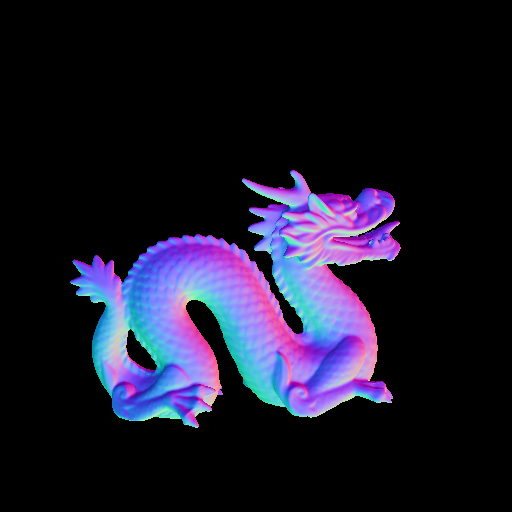
\includegraphics[width=\linewidth]{./Figures/svd-synthetic/no-noise/fancy_eval_22_groundtruth.png}
		\caption{GT}
	\end{subfigure}
	\begin{subfigure}[b]{0.32\linewidth}
		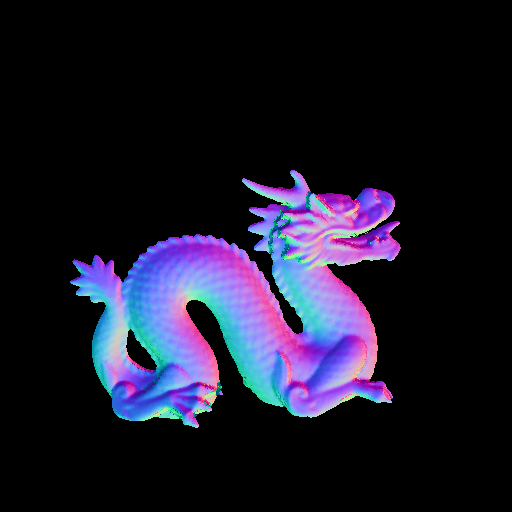
\includegraphics[width=\linewidth]{./Figures/svd-synthetic/no-noise/fancy_eval_22_normal_SVD.png}
		\caption{SVD}
	\end{subfigure}
	\begin{subfigure}[b]{0.32\linewidth}
		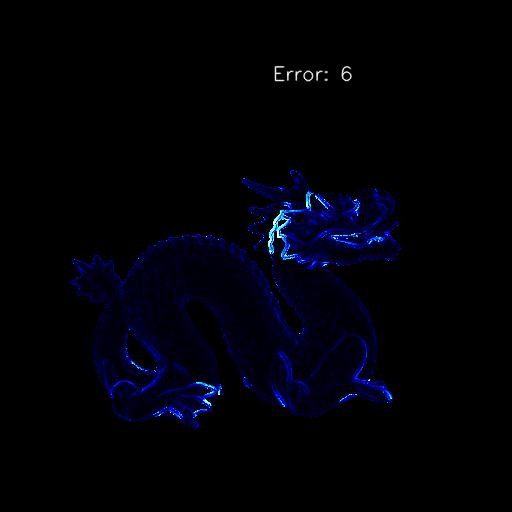
\includegraphics[width=\linewidth]{./Figures/svd-synthetic/no-noise/fancy_eval_22_error_SVD.png}
		\caption{Error}
	\end{subfigure}
	\begin{tikzpicture}
		\node[text width=0.1\textwidth] at (11,-1) {90};
		\node[inner sep=0pt] (input) at (8,-1)
		{
\includegraphics[width=.2\textwidth]{./Figures/colorscale_blue.png}};
		\node[text width=0.3\textwidth] at (7,-1) {Error: 0};
	\end{tikzpicture}
	
	\decoRule
	\caption{Normal map of a dragon object predicted by \textit{SVD}. k=1. (Resolution: $ 512\times 512 $) }
	\label{fig:svd-normal}
\end{figure}

\begin{figure}[th]
	\centering
	\captionsetup{width=\linewidth}
	\begin{subfigure}[b]{0.24\linewidth}
		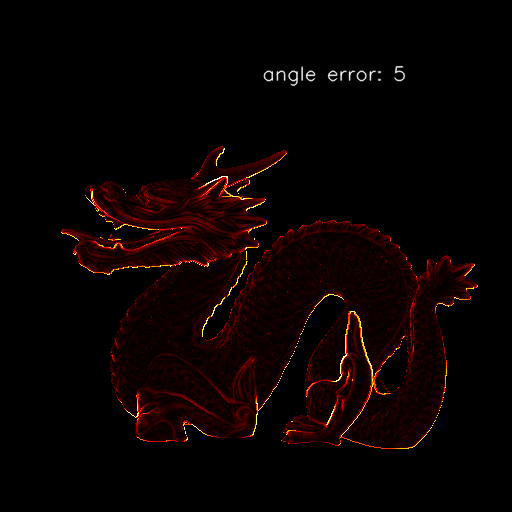
\includegraphics[width=\linewidth]{./Figures/svd-synthetic/k-compare/k1.png}
		\caption{$ k=1 $}
	\end{subfigure}
	\begin{subfigure}[b]{0.24\linewidth}
		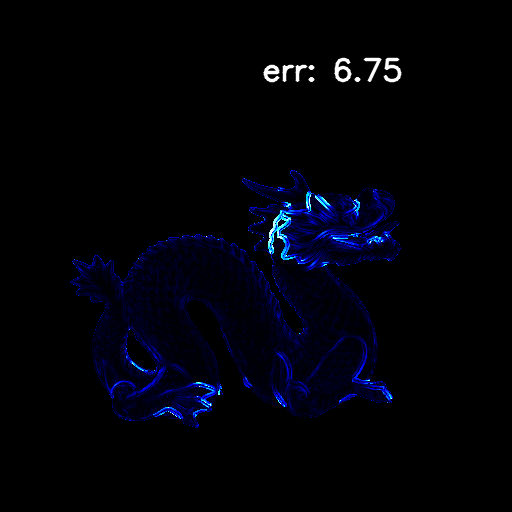
\includegraphics[width=\linewidth]{./Figures/svd-synthetic/k-compare/k2.png}
		\caption{$ k=2 $}
	\end{subfigure}
	\begin{subfigure}[b]{0.24\linewidth}
	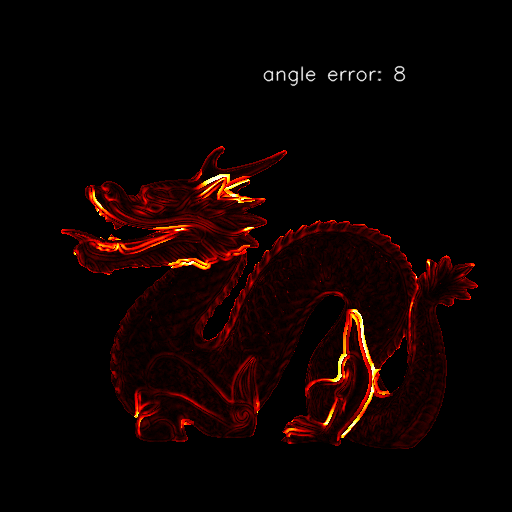
\includegraphics[width=\linewidth]{./Figures/svd-synthetic/k-compare/k3.png}
	\caption{$ k=3 $}
\end{subfigure}
	\begin{subfigure}[b]{0.24\linewidth}
	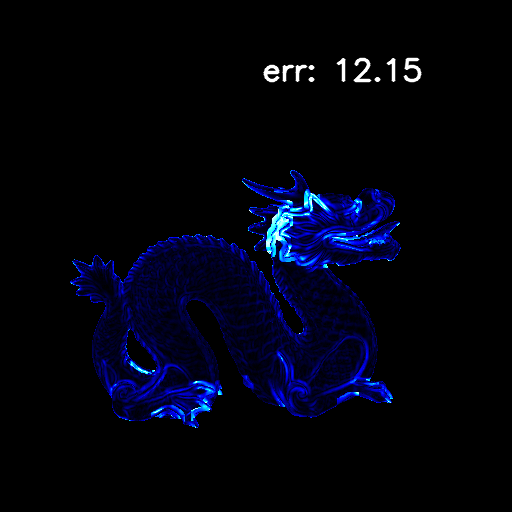
\includegraphics[width=\linewidth]{./Figures/svd-synthetic/k-compare/k4.png}
	\caption{$ k=4 $}
\end{subfigure}
	\begin{tikzpicture}
	\node[text width=0.1\textwidth] at (11,-1) {90};
	\node[inner sep=0pt] (input) at (8,-1)
	{
\includegraphics[width=.2\textwidth]{./Figures/colorscale_blue.png}};
	\node[text width=0.3\textwidth] at (7,-1) {Error: 0};
	\end{tikzpicture}
	\decoRule
	\caption{Error map of \textit{SVD} with different $ k $ values. (Resolution: $ 512\times 512 $) }
	\label{fig:svd-k-eval}
\end{figure}



\begin{figure}[H]
	\centering
	\captionsetup{width=\linewidth}
	\begin{subfigure}[b]{0.24\linewidth}
		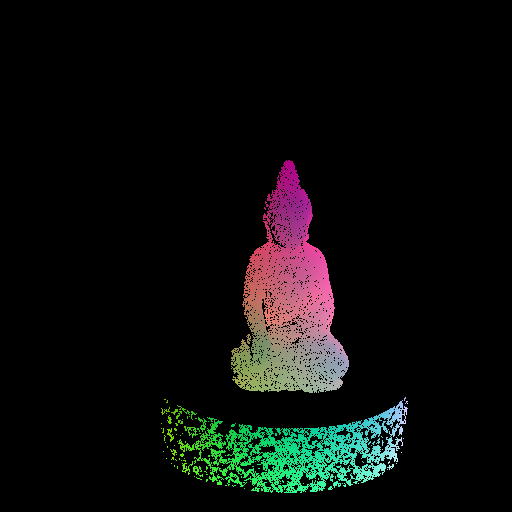
\includegraphics[width=\linewidth]{./Figures/svd-synthetic/noise/fancy_eval_0_point_cloud_noise.png}
		\caption{Vertex}
	\end{subfigure}
	\begin{subfigure}[b]{0.24\linewidth}
		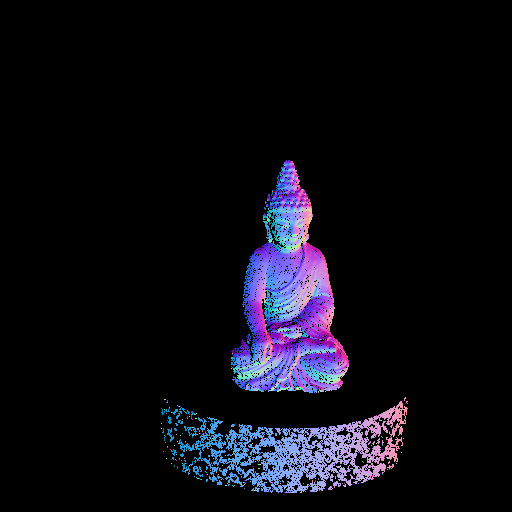
\includegraphics[width=\linewidth]{./Figures/svd-synthetic/noise/fancy_eval_0_groundtruth.png}
		\caption{GT}
	\end{subfigure}
	\begin{subfigure}[b]{0.24\linewidth}
		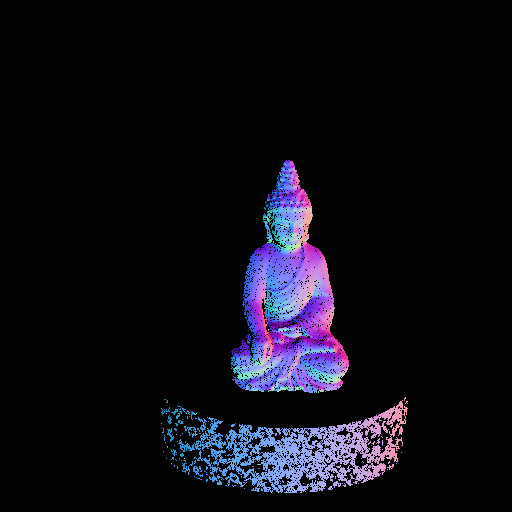
\includegraphics[width=\linewidth]{./Figures/svd-synthetic/noise/fancy_eval_0_normal_SVD.png}
		\caption{SVD}
	\end{subfigure}
	\begin{subfigure}[b]{0.24\linewidth}
		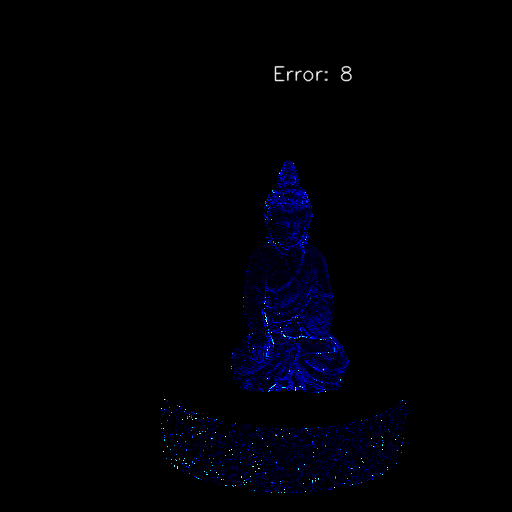
\includegraphics[width=\linewidth]{./Figures/svd-synthetic/noise/fancy_eval_0_error_SVD.png}
		\caption{Error}
	\end{subfigure}
	\begin{tikzpicture}
		\node[text width=0.1\textwidth] at (11,-1) {90};
		\node[inner sep=0pt] (input) at (8,-1)
		{
\includegraphics[width=.2\textwidth]{./Figures/colorscale_blue.png}};
		\node[text width=0.3\textwidth] at (7,-1) {Error: 0};
	\end{tikzpicture}	
	\decoRule
	\caption{\textit{SVD} visual evaluation on a noised dragon model, $ k=1 $, noise factor $ \mu $=50. (Resolution: $ 512\times 512 $) }
	\label{fig:svd-noise}
\end{figure}

The SVD approach depends on a well-chosen neighborhood size $ k $. Figure \ref{fig:svd-k-eval} shows the evaluation for different $ k $ values. For $ k=1 $, the average angle error of the whole image is the smallest, most of the normals are close to the ground truth, but the outline edges, i.e., the areas where the surface normals have changed severely. In the $ k=2 $ case, the sharp edges are smoother and cause more error, such as the eye area of the dragon. Compared to the first case, the outline edge error is better. Most of the edge errors are reduced at $ k=2 $ because more neighbor points are included in the evaluation and the effect of outliers is reduced. However, in the area of the horn outline and the hindleg outline, the error becomes worse. In this case, most of the neighbors of these points are outliers.  With $ k=3 $ and $ k=4 $, the average angular errors increase further compared to $ k=2 $.

The performance of the neighborhood-based method is good enough for a well-chosen $ k $. However, in the case of a noisy point cloud as input, this approach fails because the noise does not satisfy the neighborhood assumption and also reduces the number of possible neighbors of each point for a fixed $ k $. See figure \ref{fig:svd-noise}.



\section{Visual Evaluation on GCNN}
A qualitative evaluation on object "dragon" is shown in Figure \ref{fig:gcnn-eval}. As shown in the figure, GCNN model achieved a mean angle error in 9 degrees on this dragon object. The image has an overall good performance on the whole object. A closer evaluation is shown in Figure \ref{fig:gcnn-eval-synthetic-zoom-in}, the normal accuracy especially good on the smooth surface, like the body area. In the same case, NOC model as shown in Figure \ref{fig:gcnn-eval-multi-model} has an overall worse normal than GCNN model in the smooth area. CNN model keeps the skip connection thus gives a sharper result than NOC model, however, the overall smooth part of the model is still worse than GCNN. Besides, the sharp area like the hindleg and the head area of dragon object, CNN model gives a much brighter error map (which means a higher angle error). Figure \ref{fig:gcnn-eval-more} shows more evaluation on GCNN model.

We can get a good result from GCNN model, but from model ``Washington" we still can see it lacks the sharpness in the detail area like the face and clothes area. 


A qualitative evaluation of the object \textit{Dragon} is shown in figure \ref{fig:gcnn-eval}. As can be seen in the figure, the \textit{GCNN} model achieves an average angular error of 9 degrees for this object. The image shows an overall good performance for the whole object. A more detailed evaluation can be seen in Figure \ref{fig:gcnn-eval-synthetic-zoom-in}, the normal accuracy is especially good on the smooth surface, such as the body area. In the same case, as shown in Figure \ref{fig:gcnn-eval-multi-model}, the \textit{NOC} model has an overall worse normal than the \textit{GCNN} model in the smooth area. The \textit{CNN} model retains the skip connection and thus yields a sharper result than the \textit{NOC} model, however, the smooth region of the model is still worse overall than the \textit{GCNN} model. In addition, the \textit{CNN} model yields a much brighter error map (implying a higher angular error) in the sharp regions such as the hind leg and the head region of the dragon object. Figure \ref{fig:gcnn-eval-more} shows further evaluation of the \textit{GCNN} model on other objects.
The \textit{GCNN} model gives a good result, but for the \textit{Washington} model there is still a lack of sharpness in the detail areas such as the face and clothing. 



%% GCNN-eval
\begin{figure}[H]
	\centering
	\captionsetup{width=\linewidth}
	\begin{subfigure}[b]{0.24\linewidth}
		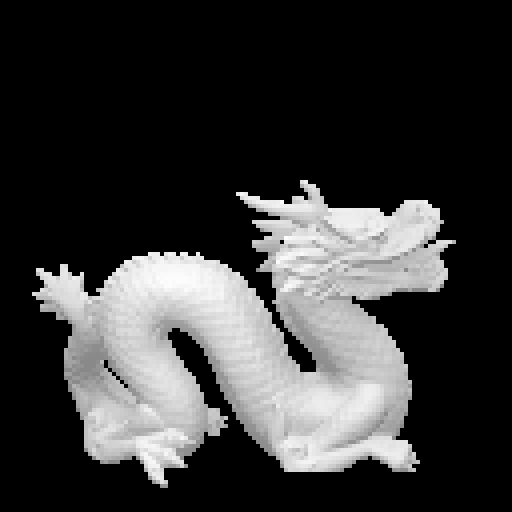
\includegraphics[width=\linewidth]{./Figures/gcnn_synthetic/fancy_eval_7_img.png}
		\caption{Image}
	\end{subfigure}
	\begin{subfigure}[b]{0.24\linewidth}
		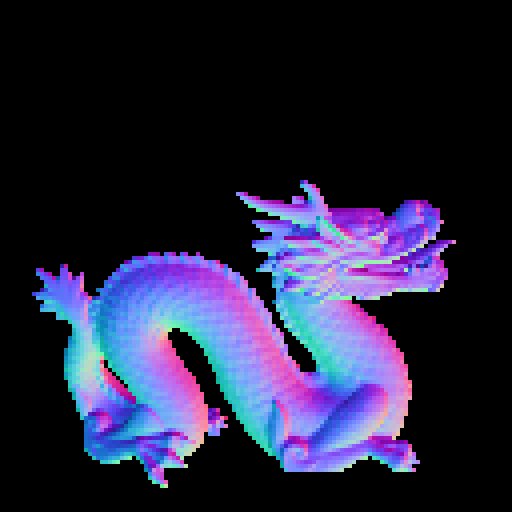
\includegraphics[width=\linewidth]{./Figures/gcnn_synthetic/fancy_eval_7_groundtruth.png}
		\caption{GT}
	\end{subfigure}
	\begin{subfigure}[b]{0.24\linewidth}
		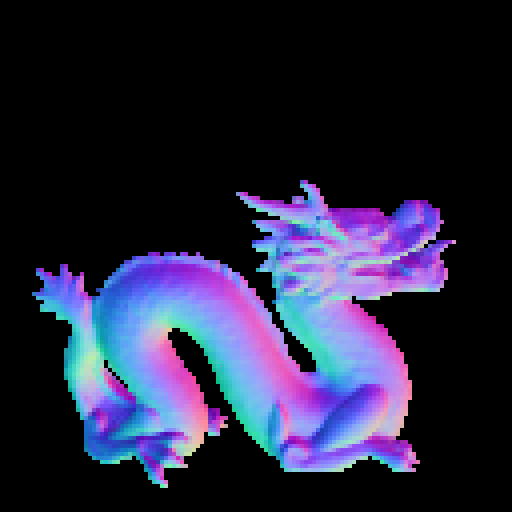
\includegraphics[width=\linewidth]{./Figures/gcnn_synthetic/fancy_eval_7_normal_GCNN-GCNN.png}
		\caption{Predict}
	\end{subfigure}
	\begin{subfigure}[b]{0.24\linewidth}
		\includegraphics[width=\linewidth]{./Figures/gcnn_synthetic/fancy_eval_7_error_GCNN.png}
		\caption{Error}
	\end{subfigure}
	
	\begin{tikzpicture}
		\node[text width=0.1\textwidth] at (11,-1) {90};
		\node[inner sep=0pt] (input) at (8,-1)
		{
\includegraphics[width=.2\textwidth]{./Figures/colorscale_blue.png}};
		\node[text width=0.3\textwidth] at (7,-1) {Error: 0};
	\end{tikzpicture}
	\decoRule
	\caption{GCNN visual evaluation. (Resolution: $ 128\times128 $)}
	\label{fig:gcnn-eval}
\end{figure}

%% GCNN zoom in eval
\begin{figure}[th]
	\centering
	\captionsetup{width=\linewidth}
	\begin{subfigure}[b]{0.18\linewidth}
		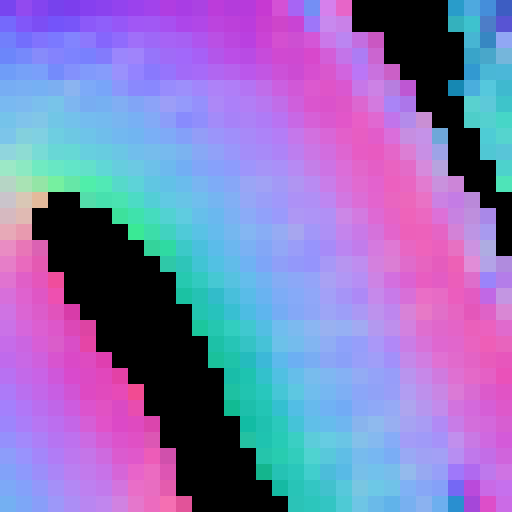
\includegraphics[width=\linewidth]{./Figures/gcnn_synthetic/eval_7_22_-8_normal.png}
	\end{subfigure}
	\begin{subfigure}[b]{0.18\linewidth}
		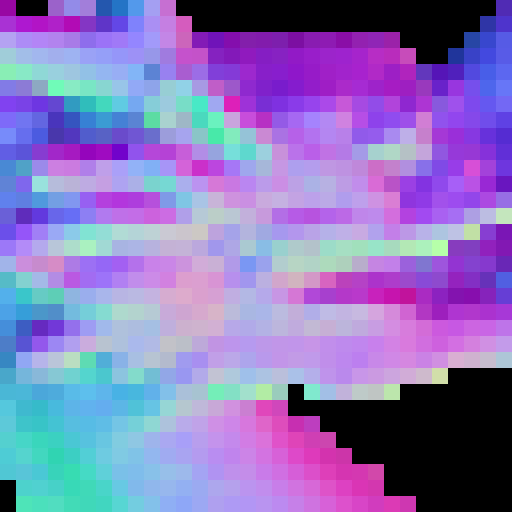
\includegraphics[width=\linewidth]{./Figures/gcnn_synthetic/eval_7_2_22_normal.png}
	\end{subfigure}
	\begin{subfigure}[b]{0.18\linewidth}
		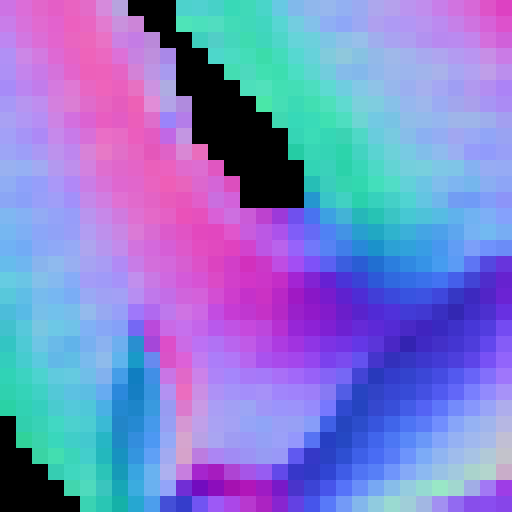
\includegraphics[width=\linewidth]{./Figures/gcnn_synthetic/eval_7_32_12_normal.png}
	\end{subfigure}
	\begin{subfigure}[b]{0.18\linewidth}
		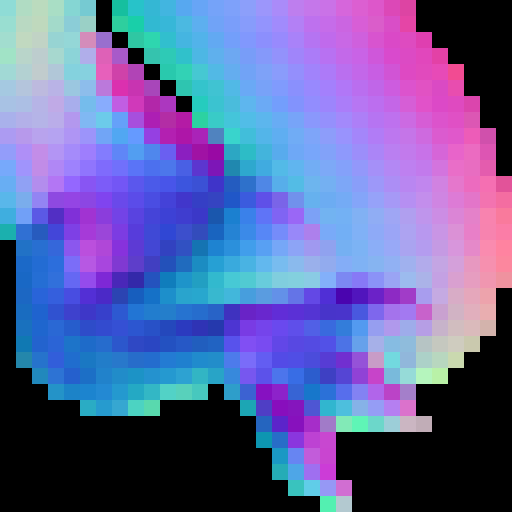
\includegraphics[width=\linewidth]{./Figures/gcnn_synthetic/eval_7_42_-28_normal.png}
	\end{subfigure}
	\begin{subfigure}[b]{0.18\linewidth}
		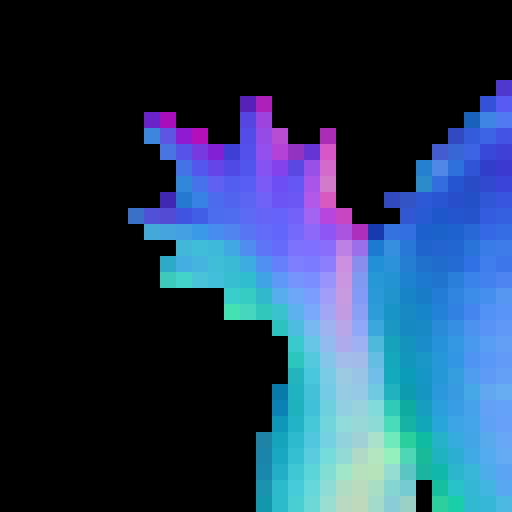
\includegraphics[width=\linewidth]{./Figures/gcnn_synthetic/eval_7_12_-48_normal.png}
	\end{subfigure}
	
	\begin{subfigure}[b]{0.18\linewidth}
		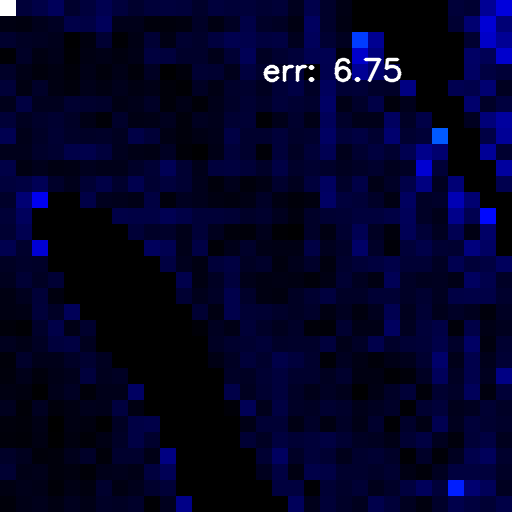
\includegraphics[width=\linewidth]{./Figures/gcnn_synthetic/eval_7_22_-8_error.png}
		\caption{Scale}
	\end{subfigure}
	\begin{subfigure}[b]{0.18\linewidth}
		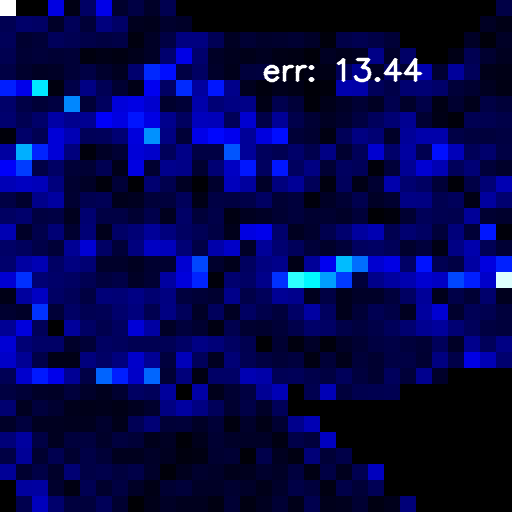
\includegraphics[width=\linewidth]{./Figures/gcnn_synthetic/eval_7_2_22_error.png}
		\caption{Head}
	\end{subfigure}
	\begin{subfigure}[b]{0.18\linewidth}
		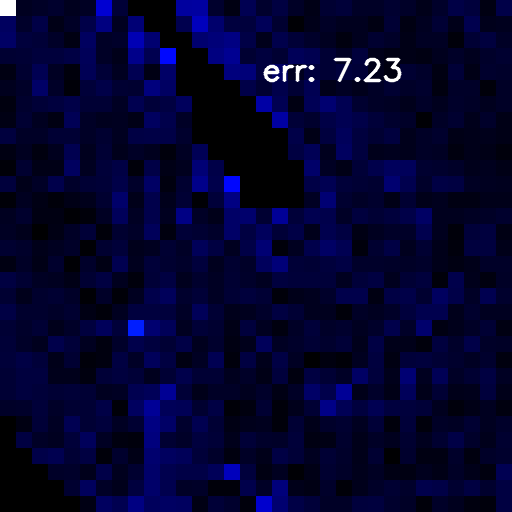
\includegraphics[width=\linewidth]{./Figures/gcnn_synthetic/eval_7_32_12_error.png}
		\caption{Foreleg}
	\end{subfigure}
	\begin{subfigure}[b]{0.18\linewidth}
		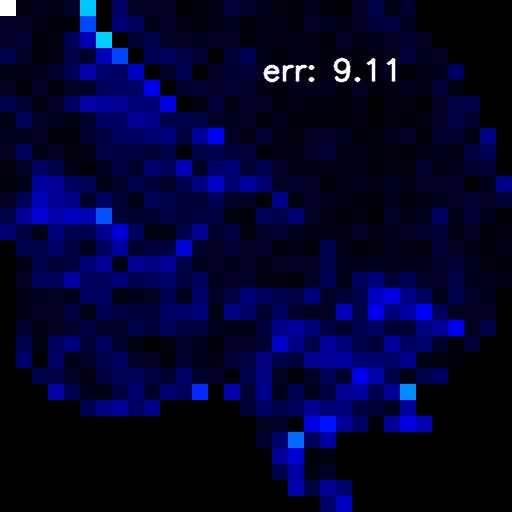
\includegraphics[width=\linewidth]{./Figures/gcnn_synthetic/eval_7_42_-28_error.png}
		\caption{Hindleg}
	\end{subfigure}
	\begin{subfigure}[b]{0.18\linewidth}
		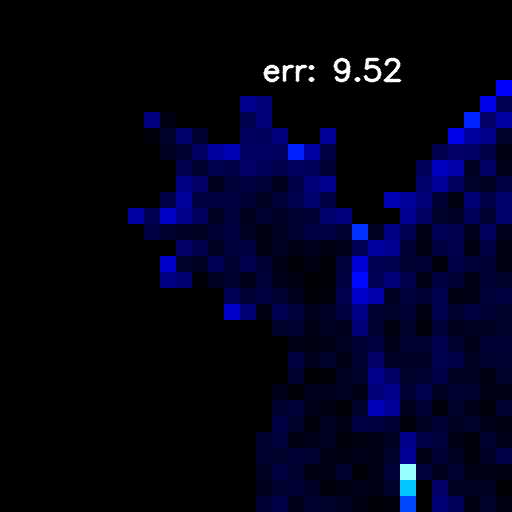
\includegraphics[width=\linewidth]{./Figures/gcnn_synthetic/eval_7_12_-48_error.png}
		\caption{Tail}
	\end{subfigure}
	
	\decoRule
	\caption{Zoom in of some regions of Dragon object (GCNN models). (Resolution: $ 32\times32 $)}
	\label{fig:gcnn-eval-synthetic-zoom-in}
\end{figure}

%% compare to other models

%% GCNN zoom in eval
\begin{figure}[H]
	\centering
	\begin{subfigure}[b]{0.24\linewidth}
		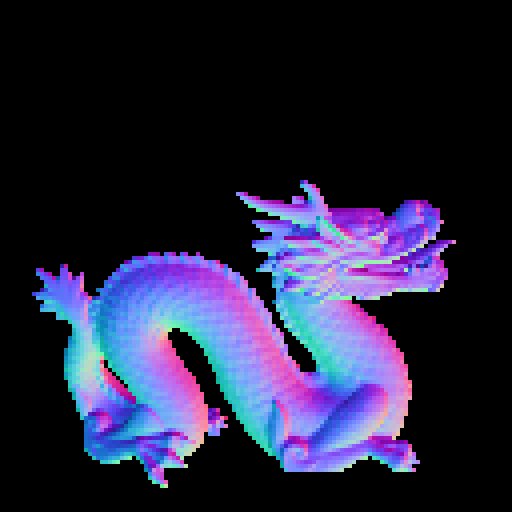
\includegraphics[width=\linewidth]{./Figures/gcnn_synthetic/fancy_eval_7_groundtruth.png}
	\end{subfigure}
	\begin{subfigure}[b]{0.24\linewidth}
		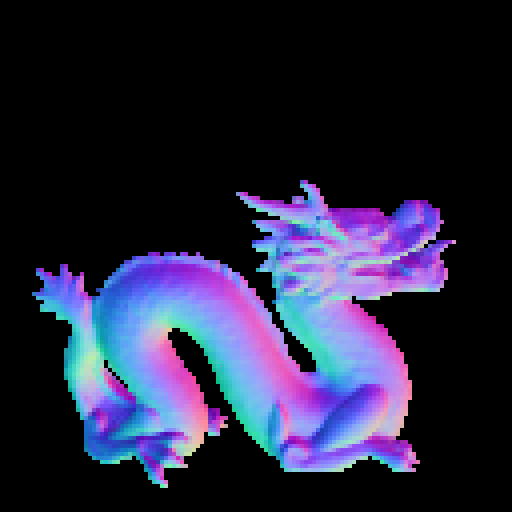
\includegraphics[width=\linewidth]{./Figures/gcnn_synthetic/fancy_eval_7_normal_GCNN-GCNN.png}
	\end{subfigure}
	\begin{subfigure}[b]{0.24\linewidth}
		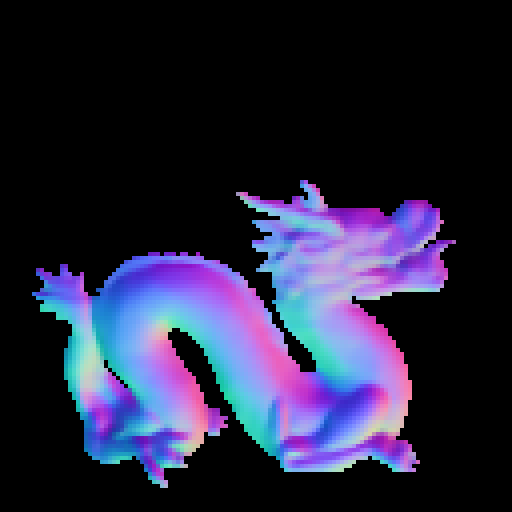
\includegraphics[width=\linewidth]{./Figures/gcnn_synthetic/fancy_eval_7_normal_GCNN-NOC.png}
	\end{subfigure}
	\begin{subfigure}[b]{0.24\linewidth}
		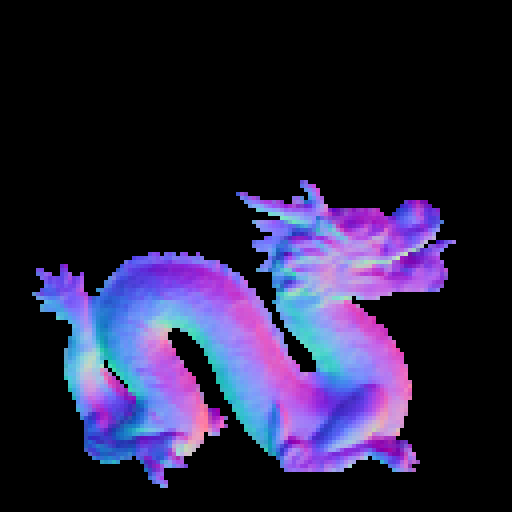
\includegraphics[width=\linewidth]{./Figures/gcnn_synthetic/fancy_eval_7_normal_GCNN-CNN.png}
	\end{subfigure}
	
	\begin{subfigure}[b]{0.24\linewidth}
		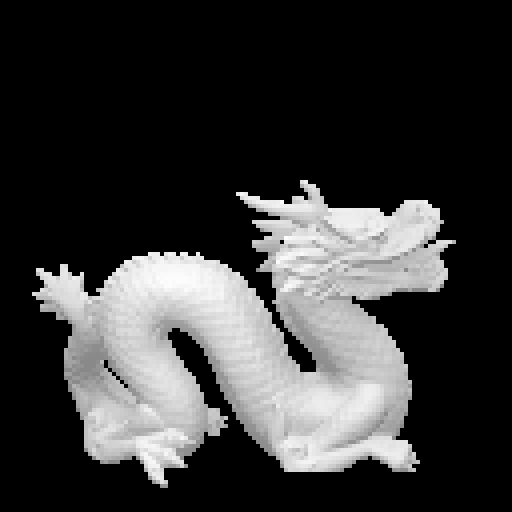
\includegraphics[width=\linewidth]{./Figures/gcnn_synthetic/fancy_eval_7_img.png}
		\caption{GT}
	\end{subfigure}
	\begin{subfigure}[b]{0.24\linewidth}
		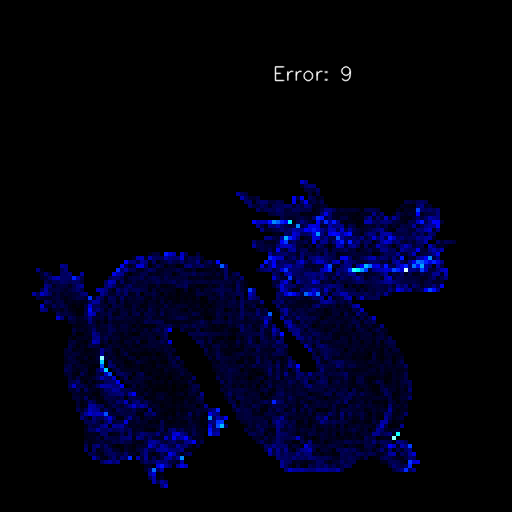
\includegraphics[width=\linewidth]{./Figures/gcnn_synthetic/fancy_eval_7_error_GCNN-GCNN.png}
		\caption{GCNN}
	\end{subfigure}
	\begin{subfigure}[b]{0.24\linewidth}
		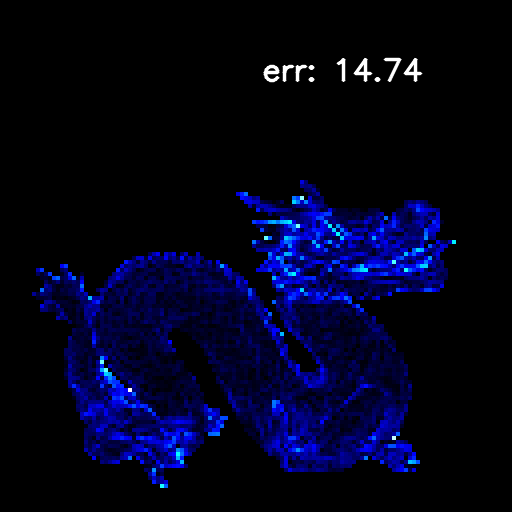
\includegraphics[width=\linewidth]{./Figures/gcnn_synthetic/fancy_eval_7_error_GCNN-NOC.png}
		\caption{NOC}
	\end{subfigure}
	\begin{subfigure}[b]{0.24\linewidth}
		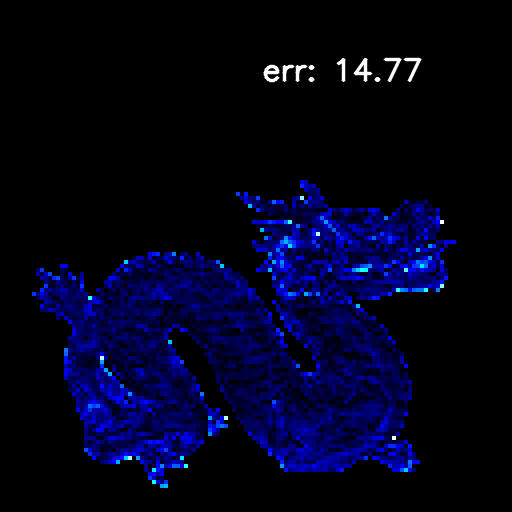
\includegraphics[width=\linewidth]{./Figures/gcnn_synthetic/fancy_eval_7_error_GCNN-CNN.png}
		\caption{CNN}
	\end{subfigure}
	
	\decoRule
	\caption{Comparison of GCNN based models. (Resolution: $ 128\times 128 $)}
	\label{fig:gcnn-eval-multi-model}
\end{figure}


\section{Discussion on the Feature Maps in GCNN}

As shown in Figure \ref{fig:gcnn-cnn-feature map}, we visualize the feature maps of the last gated convolution layer in the first upsampling part for \textit{GCNN}, \textit{NOC} and \textit{CNN} models corresponding to the 128 feature maps with size $ 32\times 32 $ in width and height. 
The input data is also the same dragon object that we used for the normal visualization. For each feature map, we assign the minimum value to the leftmost color in the color bar and the maximum value to the rightmost color in the color bar. 
We want to discuss the difference of feature maps between these three models.

To see the result clearly, we use green hue to visualize the feature maps and use brightness to distinguish the scale of the values: White corresponds to 1, Black corresponds to 0, and the colors with green hue correspond to some values in between. 

\begin{figure}[H]
	\centering
	\captionsetup{width=\linewidth}
	\begin{subfigure}[b]{0.19\linewidth}
		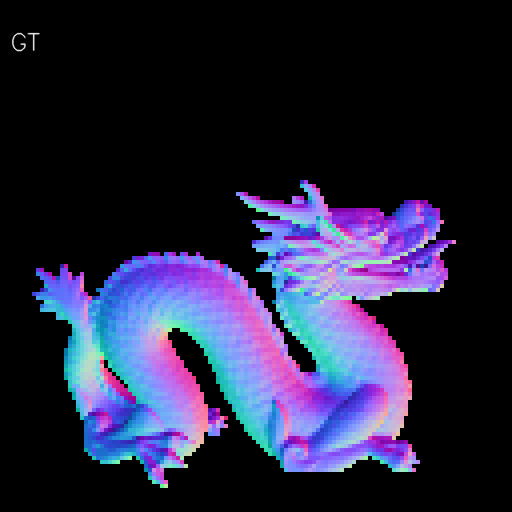
\includegraphics[width=\linewidth]{./Figures/feature_map_gcnn/feature_map_normal_gcnn-cnn.png}
		\caption{Normal Map}
	\end{subfigure}
	\begin{subfigure}[b]{0.19\linewidth}
		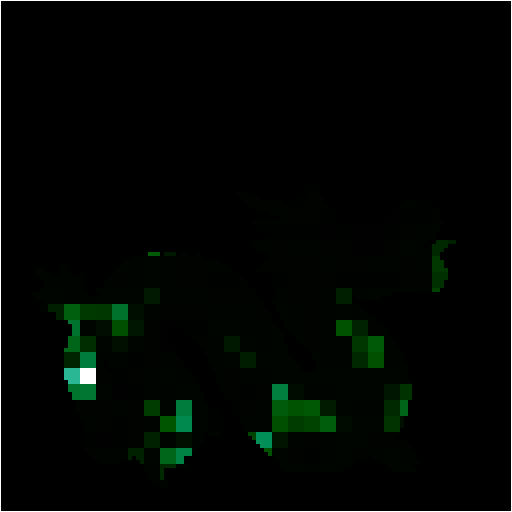
\includegraphics[width=\linewidth]{./Figures/feature_map_gcnn/feature_map_gcnn-cnn_46.png}
		\caption{Feature Map}
	\end{subfigure}
	\begin{subfigure}[b]{0.19\linewidth}
		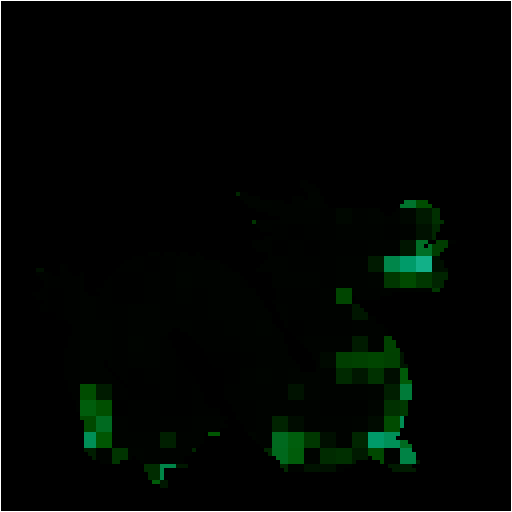
\includegraphics[width=\linewidth]{./Figures/feature_map_gcnn/feature_map_gcnn-cnn_11.png}
		\caption{Feature Map}
	\end{subfigure}
	\begin{subfigure}[b]{0.19\linewidth}
		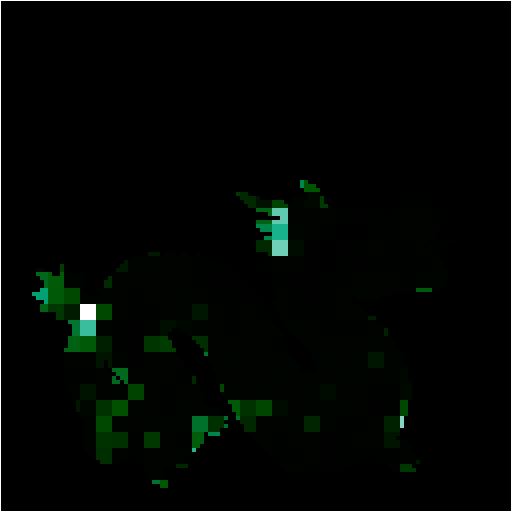
\includegraphics[width=\linewidth]{./Figures/feature_map_gcnn/feature_map_gcnn-cnn_4.png}
		\caption{Feature Map}
	\end{subfigure}
	\begin{subfigure}[b]{0.19\linewidth}
		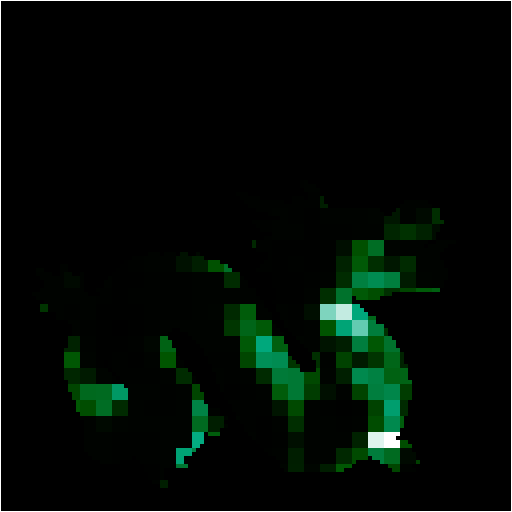
\includegraphics[width=\linewidth]{./Figures/feature_map_gcnn/feature_map_gcnn-cnn_2.png}
		\caption{Feature Map}
	\end{subfigure}
	
	\begin{tikzpicture}
		\node[text width=0.1\textwidth] at (11,-1) {1};
		\node[inner sep=0pt] (input) at (8,-1)
		{\includegraphics[width=.2\textwidth]{./Figures/colorscale_deepgreen.jpg}};
		\node[text width=0.3\textwidth] at (7,-1) {Value: 0};
	\end{tikzpicture}
	\decoRule
	\caption{Some of feature maps of CNN model in up-sampling part on resolution $ 32\times32 $}
	\label{fig:detail-feature-maps}
\end{figure}



\begin{figure}[H]
	\centering
	\captionsetup{width=\linewidth}
	\begin{subfigure}[b]{0.19\linewidth}
		\includegraphics[width=\linewidth]{./Figures/feature_map_gcnn/feature_map_out_gcnn-noc.png}
		\caption{Normal Map}
	\end{subfigure}
	\begin{subfigure}[b]{0.19\linewidth}
		\includegraphics[width=\linewidth]{./Figures/feature_map_gcnn/feature_map_gcnn-noc_39.png}
		\caption{Feature Map}
	\end{subfigure}
	\begin{subfigure}[b]{0.19\linewidth}
		\includegraphics[width=\linewidth]{./Figures/feature_map_gcnn/feature_map_gcnn-noc_45.png}
		\caption{Feature Map}
	\end{subfigure}
	\begin{subfigure}[b]{0.19\linewidth}
		\includegraphics[width=\linewidth]{./Figures/feature_map_gcnn/feature_map_gcnn-noc_93.png}
		\caption{Feature Map}
	\end{subfigure}
	\begin{subfigure}[b]{0.19\linewidth}
		\includegraphics[width=\linewidth]{./Figures/feature_map_gcnn/feature_map_gcnn-noc_104.png}
		\caption{Feature Map}
	\end{subfigure}
	
	\begin{tikzpicture}
		\node[text width=0.1\textwidth] at (11,-1) {1};
		\node[inner sep=0pt] (input) at (8,-1)
		{\includegraphics[width=.2\textwidth]{./Figures/colorscale_deepgreen.jpg}};
		\node[text width=0.3\textwidth] at (7,-1) {Value: 0};
	\end{tikzpicture}
	\decoRule
	\caption{Some of feature maps of NOC model in up-sampling part on resolution $ 32\times32 $}
	\label{fig:detail-feature-maps}
\end{figure}




\begin{figure}[H]
	\centering
	\captionsetup{width=\linewidth}
	\begin{subfigure}[b]{0.19\linewidth}
		\includegraphics[width=\linewidth]{./Figures/feature_map_gcnn/feature_map_out_gcnn-gcnn.png}
		\caption{Normal Map}
	\end{subfigure}
	\begin{subfigure}[b]{0.19\linewidth}
		\includegraphics[width=\linewidth]{./Figures/feature_map_gcnn/feature_map_gcnn-gcnn_4.png}
		\caption{Feature Map}
	\end{subfigure}
	\begin{subfigure}[b]{0.19\linewidth}
		\includegraphics[width=\linewidth]{./Figures/feature_map_gcnn/feature_map_gcnn-gcnn_5.png}
		\caption{Feature Map}
	\end{subfigure}
	\begin{subfigure}[b]{0.19\linewidth}
		\includegraphics[width=\linewidth]{./Figures/feature_map_gcnn/feature_map_gcnn-gcnn_15.png}
		\caption{Feature Map}
	\end{subfigure}
	\begin{subfigure}[b]{0.19\linewidth}
		\includegraphics[width=\linewidth]{./Figures/feature_map_gcnn/feature_map_gcnn-gcnn_127.png}
		\caption{Feature Map}
	\end{subfigure}
	
	\begin{tikzpicture}
		\node[text width=0.1\textwidth] at (11,-1) {1};
		\node[inner sep=0pt] (input) at (8,-1)
		{\includegraphics[width=.2\textwidth]{./Figures/colorscale_deepgreen.jpg}};
		\node[text width=0.3\textwidth] at (7,-1) {Value: 0};
	\end{tikzpicture}
	\decoRule
	\caption{Some of feature maps of GCNN model in up-sampling part on resolution $ 32\times32 $}
	\label{fig:detail-feature-maps}
\end{figure}

\begin{figure}[H]
		\centering
		\captionsetup{width=\linewidth}
		\begin{minipage}{0.32\linewidth}
				\begin{subfigure}[t]{0.45\linewidth}
					\includegraphics[width=\linewidth]{./Figures/feature_map_gcnn/feature_map_gcnn-cnn_113.png}
				\end{subfigure}
				\begin{subfigure}[t]{0.45\linewidth}
					\includegraphics[width=\linewidth]{./Figures/feature_map_gcnn/feature_map_gcnn-cnn_102.png}
				\end{subfigure}
			
				\begin{subfigure}[t]{0.45\linewidth}
					\includegraphics[width=\linewidth]{./Figures/feature_map_gcnn/feature_map_gcnn-cnn_65.png}
					\caption{CNN}
				\end{subfigure}
				\begin{subfigure}[t]{0.45\linewidth}
				\includegraphics[width=\linewidth]{./Figures/feature_map_gcnn/feature_map_gcnn-cnn_28.png}
				\end{subfigure}
		\end{minipage}
		\begin{minipage}{0.32\linewidth}
				\begin{subfigure}[t]{0.45\linewidth}
					\includegraphics[width=\linewidth]{./Figures/feature_map_gcnn/feature_map_gcnn-noc_7.png}
				\end{subfigure}
				\begin{subfigure}[t]{0.45\linewidth}
					\includegraphics[width=\linewidth]{./Figures/feature_map_gcnn/feature_map_gcnn-noc_25.png}
				\end{subfigure}
			
				\begin{subfigure}[t]{0.45\linewidth}
					\includegraphics[width=\linewidth]{./Figures/feature_map_gcnn/feature_map_gcnn-noc_11.png}
					\caption{NOC}
				\end{subfigure}
				\begin{subfigure}[t]{0.45\linewidth}
				\includegraphics[width=\linewidth]{./Figures/feature_map_gcnn/feature_map_gcnn-noc_127.png}
				\end{subfigure}
			
		\end{minipage}
		\begin{minipage}{0.32\linewidth}
				\begin{subfigure}[t]{0.45\linewidth}
					\includegraphics[width=\linewidth]{./Figures/feature_map_gcnn/feature_map_gcnn-gcnn_1.png}
				\end{subfigure}
				\begin{subfigure}[t]{0.45\linewidth}
					\includegraphics[width=\linewidth]{./Figures/feature_map_gcnn/feature_map_gcnn-gcnn_9.png}
				\end{subfigure}
			
				\begin{subfigure}[t]{0.45\linewidth}
					\includegraphics[width=\linewidth]{./Figures/feature_map_gcnn/feature_map_gcnn-gcnn_24.png}
					\caption{GCNN}
				\end{subfigure}
					\begin{subfigure}[t]{0.45\linewidth}
				\includegraphics[width=\linewidth]{./Figures/feature_map_gcnn/feature_map_gcnn-gcnn_75.png}
				\end{subfigure}
			
		\end{minipage}
	
		\begin{tikzpicture}
			\node[text width=0.1\textwidth] at (11,-1) {1};
			\node[inner sep=0pt] (input) at (8,-1)
			{\includegraphics[width=.2\textwidth]{./Figures/colorscale_deepgreen.jpg}};
			\node[text width=0.3\textwidth] at (7,-1) {Value: 0};
		\end{tikzpicture}
		\decoRule
		\caption{Some of feature maps of GCNN model in up-sampling part on resolution $ 32\times32 $}
		\label{fig:global-feature-maps}
\end{figure}





From the CNN feature maps, we can see that the high-value areas usually represent more than one in a single feature map. Many of them have more than two bright areas. 
In the GCNN feature maps, the bright areas are usually concentrated in only one area or even one point. When we map the bright areas onto the original image, they correspond to the dense, sharp areas, such as the mouse, horn, or tail of the kite object, which are usually the most difficult areas for the normal estimation task. We assume that these feature maps with few bright areas or only one bright area are the detail feature maps from which sharp edges can be inferred. Based on this assumption, we can say that the gated convolution layer describes the detail features more accurately compared to the standard convolution layer because the brightness regions are smaller. Most GCNN feature maps have only one bright pixel with a few green pixels, while CNN feature maps have more bright pixels with many dark pixels around the image. This accurate feature extraction gives our GCNN model better performance in the detailed areas.

Second, with the GCNN model, we found that some feature maps have very uniformly bright areas across the entire object. They are either dark overall or bright overall. Nevertheless, these feature maps differ from the detail feature maps with only a few pixels with high values (brightness), but most other pixels with relatively low values. We suspect that these uniformly distributed feature maps are the global feature maps that provide an overview of the objects for rough prediction. Thus, they can cooperate with detailed feature maps to further refine the prediction. This is also true for the NOC model since it does not have skip connections and most of the feature maps are global feature maps, so the corresponding normal maps predicted by the NOC model are coarser than those of the GCNN model. For the CNN model, there are also global feature maps, but most of them are incomplete because either the tails or the paws are missing. 
These missing areas are usually found in the detail feature maps. This also explains why the CNN detail feature maps have several bright areas in their detail feature maps. The detail feature maps and the global feature maps are mixed together. And this unclear feature map extractor leads to a decrease in performance in normal estimation tasks.




\newpage 
\section{Visual Evaluation on Trip-Net}
In the approach that uses an illuminated, calibrated RGBD image, the task is performed by the Trip-Net presented in \ref{sec:trip-net}. Based on illumination and geometry information, the Trip-Net achieves a sharper and more accurate result compared to the GCNN model.


%% TripNet-eval
\begin{figure}[H]
	\centering
	\captionsetup{width=\linewidth}
	\begin{subfigure}[b]{0.24\linewidth}
		\includegraphics[width=\linewidth]{./Figures/gcnn_synthetic/fancy_eval_7_img.png}
		\caption{Image}
	\end{subfigure}
	\begin{subfigure}[b]{0.24\linewidth}
		\includegraphics[width=\linewidth]{./Figures/gcnn_synthetic/fancy_eval_7_groundtruth.png}
		\caption{GT}
	\end{subfigure}
	\begin{subfigure}[b]{0.24\linewidth}
		\includegraphics[width=\linewidth]{./Figures/gcnn_synthetic/fancy_eval_7_normal_an2-8-1000.png}
		\caption{Predict}
	\end{subfigure}
	\begin{subfigure}[b]{0.24\linewidth}
		\includegraphics[width=\linewidth]{./Figures/gcnn_synthetic/fancy_eval_7_error_an2-8-1000.png}
		\caption{Error}
	\end{subfigure}
	
	\begin{tikzpicture}
		\node[text width=0.1\textwidth] at (11,-1) {90};
		\node[inner sep=0pt] (input) at (8,-1)
		{\includegraphics[width=.2\textwidth]{./Figures/colorscale_blue.png}};
		\node[text width=0.3\textwidth] at (7,-1) {Error: 0};
	\end{tikzpicture}
	\decoRule
	\caption{Trip-Net visual evaluation on resolution $ 128\times128 $}
	\label{fig:trip-eval}
\end{figure}
The qualitative evaluation is shown in Figure \ref{fig:trip-eval}. To show the effectiveness of the added illuminated information, the training settings are exactly the same for all models. We also use the same inputs as for the GCNN evaluation. The error of the Trip-Net is $ 6^\circ $, and that of the GCNN is $ 9^\circ $. 

%% tripNet zoom in eval
\begin{figure}[H]
	\centering
	\captionsetup{width=\linewidth}
	\begin{subfigure}[b]{0.18\linewidth}
		\includegraphics[width=\linewidth]{./Figures/trip_net_zoom_in/eval_7_22_-8_normal.png}
	\end{subfigure}
	\begin{subfigure}[b]{0.18\linewidth}
		\includegraphics[width=\linewidth]{./Figures/trip_net_zoom_in/eval_7_2_22_normal.png}
	\end{subfigure}
	\begin{subfigure}[b]{0.18\linewidth}
		\includegraphics[width=\linewidth]{./Figures/trip_net_zoom_in/eval_7_32_12_normal.png}
	\end{subfigure}
	\begin{subfigure}[b]{0.18\linewidth}
		\includegraphics[width=\linewidth]{./Figures/trip_net_zoom_in/eval_7_42_-28_normal.png}
	\end{subfigure}
	\begin{subfigure}[b]{0.18\linewidth}
		\includegraphics[width=\linewidth]{./Figures/trip_net_zoom_in/eval_7_12_-48_normal.png}
	\end{subfigure}
	
	\begin{subfigure}[b]{0.18\linewidth}
		\includegraphics[width=\linewidth]{./Figures/trip_net_zoom_in/eval_7_22_-8_error.png}
		\caption{Scale}
	\end{subfigure}
	\begin{subfigure}[b]{0.18\linewidth}
		\includegraphics[width=\linewidth]{./Figures/trip_net_zoom_in/eval_7_2_22_error.png}
		\caption{Head}
	\end{subfigure}
	\begin{subfigure}[b]{0.18\linewidth}
		\includegraphics[width=\linewidth]{./Figures/trip_net_zoom_in/eval_7_32_12_error.png}
		\caption{Foreleg}
	\end{subfigure}
	\begin{subfigure}[b]{0.18\linewidth}
		\includegraphics[width=\linewidth]{./Figures/trip_net_zoom_in/eval_7_42_-28_error.png}
		\caption{Hindleg}
	\end{subfigure}
	\begin{subfigure}[b]{0.18\linewidth}
		\includegraphics[width=\linewidth]{./Figures/trip_net_zoom_in/eval_7_12_-48_error.png}
		\caption{Tail}
	\end{subfigure}
	
	\decoRule
	\caption{Zoom in of detail regions ($ 32\times32 $) of \textit{Dragon} object (Trip-Net).}
	\label{fig:tripnet-eval-synthetic-zoom-in}
\end{figure}

As can be seen in the Figure \ref{fig:tripnet-eval-synthetic-zoom-in}, the scale of the dragon's body is much easier to see and is also closer to the ground truth. The head region provides a sharper edge prediction. All five sampled zoom-in regions in Trip-Net have better performance than GCNN. 


Figure \ref{fig:tripnet-fusion-eval} compares different fusion times on the Trip-Net model. It can be seen that the F1 with one fusion and F2 with two fusions models do not perform better compared to the GCNN model, which means that the illuminated information does not work when we consider only the lower resolution feature maps. The F3 model with three fusions and the F4 model with four fusions provide a much better result and also outperform the GCNN model. In these two fusion models, the high-resolution features are included. We can observe the dragon scale in the figures, it is much sharper in F3 and F4.

%% F1-F4 eval

\begin{figure}
	\centering
	\captionsetup{width=\linewidth}
	\begin{subfigure}[b]{0.18\linewidth}
		\includegraphics[width=\linewidth]{./Figures/gcnn_synthetic/fancy_eval_7_groundtruth.png}
	\end{subfigure}
	\begin{subfigure}[b]{0.18\linewidth}
		\includegraphics[width=\linewidth]{./Figures/gcnn_synthetic/fancy_eval_7_normal_f1.png}
	\end{subfigure}
	\begin{subfigure}[b]{0.18\linewidth}
		\includegraphics[width=\linewidth]{./Figures/gcnn_synthetic/fancy_eval_7_normal_f2.png}
	\end{subfigure}
	\begin{subfigure}[b]{0.18\linewidth}
		\includegraphics[width=\linewidth]{./Figures/gcnn_synthetic/fancy_eval_7_normal_f3.png}
	\end{subfigure}
	\begin{subfigure}[b]{0.18\linewidth}
		\includegraphics[width=\linewidth]{./Figures/gcnn_synthetic/fancy_eval_7_normal_f4.png}
	\end{subfigure}
	
	
	\begin{subfigure}[b]{0.18\linewidth}
		\includegraphics[width=\linewidth]{./Figures/gcnn_synthetic/fancy_eval_7_img.png}
		\caption{GT}
	\end{subfigure}
	\begin{subfigure}[b]{0.18\linewidth}
		\includegraphics[width=\linewidth]{./Figures/gcnn_synthetic/fancy_eval_7_error_f1.png}
		\caption{F1}
	\end{subfigure}
	\begin{subfigure}[b]{0.18\linewidth}
		\includegraphics[width=\linewidth]{./Figures/gcnn_synthetic/fancy_eval_7_error_f2.png}
		\caption{F2}
	\end{subfigure}
	\begin{subfigure}[b]{0.18\linewidth}
		\includegraphics[width=\linewidth]{./Figures/gcnn_synthetic/fancy_eval_7_error_f3.png}
		\caption{F3}
	\end{subfigure}
	\begin{subfigure}[b]{0.18\linewidth}
		\includegraphics[width=\linewidth]{./Figures/gcnn_synthetic/fancy_eval_7_error_f4.png}
		\caption{F4}
	\end{subfigure}
	
	\decoRule
	\caption{Comparison between different fusion times on Trip-Net Architecture ($ 128\times128 $). }
	\label{fig:tripnet-fusion-eval}
\end{figure}




\section{Trining on Higher Resolution}
We also trained our models on a higher resolution dataset with $ 512 \times 512 $ in width and height for each scene. Higher resolution data provides more information about surface features using the same model compared to lower resolutions. The advantage is that if we extract a fixed size patch from the normal map, say $32\times32$, it may correspond to a hind leg of the dragon object at a resolution of $128 \times 128$ scene, but at a resolution of $512\times 512$ scene, it may only correspond to a toe. Thus, if we still use the same kernel size in the network for the same data set (as in $ 3\times 3 $), the higher the resolution, the smaller the corresponding surface area. 
Thus, for the higher resolution, the surface becomes smoother and the surface normal can be computed more easily in a fixed size of area compare to lower resolution. This is a good thing. Because then we may only need to use these $ 32\ times 32 $ points to calculate a toe in an image with $ 512\ times512 $ resolution. But in an image with a resolution of $ 128\times128 $, the same area $ 32\times32 $ could correspond to the entire hind leg of the dragon object. In other words. Thus, the higher resolution helps the model to compute a more accurate normal map. 


%% 5 degree metric
\begin{table}[H]
	\centering
	\captionsetup{width=\linewidth}
	\begin{tabular}{l | l l l }
		\toprule
		\tabhead{Metrics} & \tabhead{SVD} & \tabhead{GCNN} & \tabhead{Trip-Net} \\
		\midrule
		Mean  					& 8.88 & 5.82 & 5.33 \\ 
		\hline
		Median					& 3.66 & 3.98 & 3.67 \\ 
		\hline
		$ 5^\circ $ 			& 0.63 & 0.63 & 0.66 \\
		\hline
		$ 11.5^\circ $ 			& 0.79 & 0.89 & 0.91 \\
		\hline
		$ 22.5^\circ $ 			& 0.89 & 0.97 & 0.97 \\
		\hline
		$ 30^\circ $ 			& 0.92 & 0.98 & 0.99 \\
		\bottomrule
	\end{tabular}
	\caption{High resolution dataset evaluation of SVD, GCNN and Trip-Net models on 6 different metrics based on 100 test scenes. (Resolution: $ 512\times512 $)}	
	\label{tab:high_resolution_eval}
\end{table}

Since our model is a fully convolutional network, the architecture remains exactly the same on the high-resolution dataset. We use the same settings and the same model for training on a $ 512\times512 $ resolution dataset. Training with the high-resolution network takes longer, but results in a lower angular error. 



%% high resolution trip-net visualization
\begin{figure}[th]
	\centering
	\captionsetup{width=\linewidth}
	\begin{subfigure}[b]{0.48\linewidth}
		\includegraphics[width=\linewidth]{./Figures/comparison_512/fancy_eval_11_normal_Trip-Net-512.png}
		\caption{Trip-Net}
	\end{subfigure}
	\begin{subfigure}[b]{0.48\linewidth}
		\includegraphics[width=\linewidth]{./Figures/comparison_512/fancy_eval_11_groundtruth.png}
		\caption{GT}
	\end{subfigure}
	
	
	\begin{subfigure}[b]{0.32\linewidth}
		\includegraphics[width=\linewidth]{./Figures/comparison_512/fancy_eval_11_point_cloud_noise.png}
		\caption{Input}
	\end{subfigure}
	\begin{subfigure}[b]{0.32\linewidth}
		\includegraphics[width=\linewidth]{./Figures/comparison_512/fancy_eval_11_img.png}
		\caption{Image}
	\end{subfigure}
	\begin{subfigure}[b]{0.32\linewidth}
		\includegraphics[width=\linewidth]{./Figures/comparison_512/fancy_eval_11_error_Trip-Net-512.png}
		\caption{Error}
	\end{subfigure}
	
	\begin{tikzpicture}
		\node[text width=0.1\textwidth] at (11,-1) {90};
		\node[inner sep=0pt] (input) at (8,-1)
		{\includegraphics[width=.2\textwidth]{./Figures/colorscale_blue.png}};
		\node[text width=0.3\textwidth] at (7,-1) {Error: 0};
	\end{tikzpicture}
	\decoRule
	\caption{Trip-Net visual evaluation on high resolution dataset $ 512 \times 512 $.}
	\label{fig:trip-eval-high-resolution}
\end{figure}







A quantitative evaluation is shown in Table \ref{tab:high_resolution_eval}. It follows the same performance ranking compared to lower resolutions, i.e. GCNN is better than the SVD approach and Trip-Net is slightly better than GCNN. The accuracy is 99\% in the $30^\circ $ metric. In the average error metric, the error is $ 5^\circ $.  A qualitative evaluation is shown in Figure \ref{fig:trip-eval-high-resolution}. We use a figure object with smooth regions (belly and arm) and highly detailed regions with sharp surfaces (the uneven surface of the stone table) for the evaluation. Our models yield a $ 5^\circ $ in the middle degree of the metric. 

A comparison with other models is shown in Figure \ref{fig:trip-eval-compare}. Note that we use the same dragon object (with slightly shifted location since they were collected at different times in the high-resolution dataset) for the assessment to allow a coherent comparison with the low-resolution dataset. The \textit{SVD} approach yields a good result ($8.88^\circ $ in the average degree metric). As mentioned earlier, the surfaces are relatively smoother when we keep the same window size for normal inference. In the high-resolution scenes, the percentage of missing pixels in a fixed window is the same as in the low-resolution scenes, but the remaining valid pixels in the same window size are on a relatively flat plane and are therefore good enough for accurate normal inference. However, as expected, we can still see the high-level error in the sharp edges of the dragon object, such as the horns and the hind leg areas, as shown in Figure \ref{fig:trip-eval-compare}.



%& trip-net evaluation with other models

\begin{figure}[th]
	\centering
	\captionsetup{width=\linewidth}
	\begin{subfigure}[b]{0.24\linewidth}
		\includegraphics[width=\linewidth]{./Figures/comparison_512/fancy_eval_14_groundtruth.png}
	\end{subfigure}
	\begin{subfigure}[b]{0.24\linewidth}
		\includegraphics[width=\linewidth]{./Figures/comparison_512/fancy_eval_14_normal_SVD.png}
	\end{subfigure}
	\begin{subfigure}[b]{0.24\linewidth}
		\includegraphics[width=\linewidth]{./Figures/comparison_512/fancy_eval_14_normal_NNNN-512.png}
	\end{subfigure}
	\begin{subfigure}[b]{0.24\linewidth}
		\includegraphics[width=\linewidth]{./Figures/comparison_512/fancy_eval_14_normal_Trip-Net-512.png}
	\end{subfigure}
	
	
	\begin{subfigure}[b]{0.24\linewidth}
		\includegraphics[width=\linewidth]{./Figures/comparison_512/fancy_eval_14_img.png}
		\caption{GT}
	\end{subfigure}
	\begin{subfigure}[b]{0.24\linewidth}
		\includegraphics[width=\linewidth]{./Figures/comparison_512/fancy_eval_14_error_SVD.png}
		\caption{SVD}
	\end{subfigure}
	\begin{subfigure}[b]{0.24\linewidth}
		\includegraphics[width=\linewidth]{./Figures/comparison_512/fancy_eval_14_error_NNNN-512.png}
		\caption{GCNN}
	\end{subfigure}
	\begin{subfigure}[b]{0.24\linewidth}
		\includegraphics[width=\linewidth]{./Figures/comparison_512/fancy_eval_14_error_Trip-Net-512.png}
		\caption{Trip-Net}
	\end{subfigure}
	\decoRule
	\caption{Comparison on high resolution dataset ($ 512\times 512 $).}
	\label{fig:trip-eval-compare}
\end{figure}


\section{Training on Real-Dataset}
We also applied our model to a dataset acquired with a structured light scanner in our laboratory to test the applicability of our model to the real dataset. For the approach based on geometry information, we directly use the GCNN model trained on synthetic datasets since it only needs the depth map as input and the scenarios of the two datasets are the same. For the approach based on illuminated calibrated RGB-D images, the model needs to be refined based on the real dataset because the light intensity, position, and camera matrix are different. We have refined the Trip-Net based on a pre-trained GCNN model with the same settings in previous experiments.


\begin{table}[H]
	\centering
	\captionsetup{width=\linewidth}
	\begin{tabular}{l | l l l }
		\toprule
		\tabhead{Metrics} & \tabhead{SVD} & \tabhead{GCNN} & \tabhead{Trip-Net} \\
		\midrule
		Mean  					& 8.20 & 8.74 & \textbf{8.09}\\ 
		\hline
		Median					& \textbf{4.87} & 5.70 & 5.00 \\ 
		\hline
		$ 5^\circ $ 			& \textbf{0.51} & 0.44 & 0.50 \\
		\hline
		$ 11.5^\circ $ 			& 0.79 & 0.79 & \textbf{0.81} \\
		\hline
		$ 22.5^\circ $ 			& 0.93 & 0.93 & \textbf{0.94} \\
		\hline
		$ 30^\circ $ 			& 0.96 & 0.96 & 0.96 \\
		\bottomrule
	\end{tabular}
	\caption{Evaluation of SVD, GCNN and Trip-Net models on 6 different metrics based on 100 test scenes in Real-Dataset.}	
	\label{tab:real_eval}
\end{table}


We do not have a ground truth for evaluation in the Real-Dataset. But if we look directly at the visualization in Figure \ref{fig:trip-eval-real}, we can see that the Trip-Net approach is well able to ``enhance'' the missing pixels in the scenes and also gives a sharp result. The wrinkles on the clothes are detectable and even countable. Figure \ref{fig:real_eval_compare} compares the trip net with other approaches.


However, we also noticed that the large holes in the base level are preserved in the Normal Maps. These large holes correspond to the shiny and dark texture regions that are often present in the depth map captured by the scanners. Since these large holes are only related to specific feature areas and also have irregular shapes, we did not simulate this type of noise in the synthetic dataset, but only with a sparse binary mask. Therefore, our models could not fill in missing large holes in the estimated normal map. Further work on this topic could be to find a way to generate a very similar depth map noise to obtain a more robust training dataset. 

\begin{figure}[th]
	\centering
	\captionsetup{width=\linewidth}
	\begin{subfigure}[b]{0.32\linewidth}
		\includegraphics[width=\linewidth]{./Figures/comparison_real/fancy_eval_20_groundtruth.png}
		\caption{GT}
	\end{subfigure}
	\begin{subfigure}[b]{0.32\linewidth}
	\includegraphics[width=\linewidth]{./Figures/comparison_real/fancy_eval_20_normal_An2_no_mask.png}
	\caption{Trip-Net}
	\end{subfigure}
	\begin{subfigure}[b]{0.32\linewidth}
		\includegraphics[width=\linewidth]{./Figures/comparison_real/fancy_eval_20_normal_An2-real-resume-616.png}
		\caption{Trip-Net (No-Mask)}
	\end{subfigure}
	
	\begin{subfigure}[b]{0.32\linewidth}
		\includegraphics[width=\linewidth]{./Figures/comparison_real/fancy_eval_20_point_cloud_noise.png}
		\caption{Input}
	\end{subfigure}
	\begin{subfigure}[b]{0.32\linewidth}
		\includegraphics[width=\linewidth]{./Figures/comparison_real/fancy_eval_22_img.png}
		\caption{Image}
	\end{subfigure}
	\begin{subfigure}[b]{0.32\linewidth}
		\includegraphics[width=\linewidth]{./Figures/comparison_real/fancy_eval_22_error_An2-real-resume.png}
		\caption{Error}
	\end{subfigure}
	
	\begin{tikzpicture}
		\node[text width=0.1\textwidth] at (11,-1) {90};
		\node[inner sep=0pt] (input) at (8,-1)
		{\includegraphics[width=.2\textwidth]{./Figures/colorscale_blue.png}};
		\node[text width=0.3\textwidth] at (7,-1) {Error: 0};
	\end{tikzpicture}
	\decoRule
	\caption{Real Dataset ($ 512\times 512 $) evaluation (Trip-Net)}
	\label{fig:trip-eval-real}
\end{figure}




%% real eval comparison
\begin{figure}[th]
	\centering
	\captionsetup{width=\linewidth}
	\begin{subfigure}[b]{0.2\linewidth}
		\includegraphics[width=\linewidth]{./Figures/comparison_real/fancy_eval_0_groundtruth.png}
	\end{subfigure}
	\begin{subfigure}[b]{0.2\linewidth}
		\includegraphics[width=\linewidth]{./Figures/comparison_real/fancy_eval_0_normal_SVD.png}
	\end{subfigure}
	\begin{subfigure}[b]{0.2\linewidth}
		\includegraphics[width=\linewidth]{./Figures/comparison_real/fancy_eval_0_normal_NNNN-512.png}
	\end{subfigure}
	\begin{subfigure}[b]{0.2\linewidth}
		\includegraphics[width=\linewidth]{./Figures/comparison_real/fancy_eval_0_normal_An2-real-resume.png}
	\end{subfigure}
	
	
	\begin{subfigure}[b]{0.2\linewidth}
		\includegraphics[width=\linewidth]{./Figures/comparison_real/00008.image0.png}
		\caption{GT}
	\end{subfigure}
	\begin{subfigure}[b]{0.2\linewidth}
		\includegraphics[width=\linewidth]{./Figures/comparison_real/fancy_eval_0_error_SVD.png}
		\caption{SVD}
	\end{subfigure}	
	\begin{subfigure}[b]{0.2\linewidth}
		\includegraphics[width=\linewidth]{./Figures/comparison_real/fancy_eval_0_error_NNNN-512.png}
		\caption{GCNN}
	\end{subfigure}
	\begin{subfigure}[b]{0.2\linewidth}
		\includegraphics[width=\linewidth]{./Figures/comparison_real/fancy_eval_0_error_An2-real-resume.png}
		\caption{Trip-Net}
	\end{subfigure}	
	\decoRule
	\caption{Real dataset ($ 512\times 512 $) comparison.}
	\label{fig:real_eval_compare}
\end{figure}
